\documentclass[12pt, onecolumn,notitlepage]{article}

    \usepackage{indentfirst}
    \usepackage{amsmath}
    \DeclareMathOperator\arctanh{arctanh}
    \usepackage{xcolor, graphicx}
    \usepackage{wrapfig}
    \usepackage{caption} 
    \captionsetup{justification=justified}
    \usepackage{appendix}
    \usepackage{textcomp}
    \usepackage{natbib}
    \usepackage[UKenglish]{babel}


    %\usepackage{datetime}
    %%%%%\usepackage[ddmmyyyy]{datetime}
    \setlength{\bibsep}{1pt}
    \setlength{\textheight}{679pt}
    \setlength{\voffset}{-2.5cm}
    \setlength{\textwidth}{17cm}
    \setlength{\hoffset}{-1.5cm}
    \graphicspath{ {./figures/} }
   

% define the title


\begin{document}

\pagenumbering{gobble}

    \begin{center}
    \vspace*{3cm}
    {\huge\bfseries Commissioning of ATLAS Flavour Tagging Algorithms in Run-2 Data \par}
    \vspace{2cm}
    {\Large Laurie M\textsuperscript{c}Clymont \par} 
    \vspace{0.5cm}
    {\Large University College London \par}
    {\Large First Year Transfer Report \par}
    \vspace{0.5cm}
    {\scshape\Large \par}
    {\large supervised by\par
    \Large Dr. Andreas Korn}
    
    \vspace{1.5cm}
    
    \begin{abstract}    
         \normalsize
         The identification of jets containing \textit{b}-hadrons or \textit{c}-hadrons, known as flavour tagging,
         is an important part of the Run-2 physics program at the ATLAS experiment.
         For example it features in searches for beyond standard model physics,
         such as the proposed analysis using the dijet mass spectrum of
         two \textit{b}-tagged jets presented in this report.
         For Run-2, there have been many changes that affect flavour tagging; the increase in centre-of-mass energy, the introduction of a new inner-most tracking layer 
         and changes to the algorithms used for flavour tagging.
         In this report flavour tagging in Run-2 is validated by comparing distributions of
         variables relevant to flavour tagging in early Run-2 data from ATLAS to Monte Carlo simulation.
         Also presented in this report is a study into improving high-$p_T$ \textit{b}-tagging by introducing a new track-$p_T$ cut that depends on
         jet-$p_T$.
         
    \end{abstract}

    %\includegraphics[width=0.15\textwidth]{example-image-1x1}\par\vspace{1cm}


    \vfill

    % Bottom of the page
    {\large \today\par}
    \end{center}
\newpage


\pagenumbering{arabic}

\section*{Introduction} \label{s_Intro}

In high energy proton collisions, narrow beams of propagating high energy hadrons, known as  jets,  are produced by interactions that 
contain free quarks or gluons in their final states. 
Flavour tagging is the identification of \textit{b}-jets, \textit{c}-jets and light-flavoured jets, which are defined as jets containing a \textit{b}-hadron, 
a charmed-hadron or only light hadrons (only containing \textit{u},\textit{d} and \textit{s} quarks) respectively.
Flavour tagging is performed by algorithms that utilise the long lifetimes (of the order ps) of the heavy-hadrons that decay through the flavour changing weak interaction,
of which a \textit{b}- or \textit{c}-jet must contain at least one as, 
at the quark level, the \textit{b} or \textit{c} quark contained in the jet must undergo a flavour change.
The long lifetimes of the heavy flavour hadrons means that they will decay a measurable distance from the 
primary vertex, the point where the hard-scatter collision occurs, and hence the flavour can be inferred from the presence of particles 
that originate from a point offset from the primary vertex. \\

Following the first run of data taking at ATLAS in 2010-12, Run-1, there has been a long shutdown in preparation for the second run of data taking, Run-2, 
at a higher collision energy of $\sqrt{s} = 13$ TeV, which began in May 2015.
During the long shutdown there have been many changes to the ATLAS detector and to flavour tagging algorithms that have an effect on flavour tagging. 
The performance of flavour tagging after these changes has been tested and optimised in Monte Carlo simulations of 13 TeV collisions at the ATLAS detector,
and it has been shown that there are improvements in flavour tagging performance in the simulations \cite{bib_Run2_perf}.
However, it is important that the understanding of flavour tagging performance gained in simulation is validated in data before Run-2 flavour tagging can 
be used in analyses. 
This is done by comparing the distributions of the key variables relevant to flavour tagging in data and simulation. 
This study uses events containing two or more jets, known as an inclusive dijet sample. \\

Flavour tagging of \textit{b}-quarks (\textit{b}-tagging) is important for many analyses.
Two important analyses where \textit{b}-tagging features strongly are $t\bar{t}$ analyses \cite{bib_ttbar}
and searches for a Higgs boson decaying to $b\bar{b}$ \cite{bib_Hbb}.
In the former, as the top decays to a \textit{W}-boson and a \textit{b}-quark with a branching ratio close to 100\%, 
$t\bar{t}$ analyses typically require \textit{b}-tagged jets in the event. 
In the latter, the Higgs boson coupling is proportional to mass squared, hence the large mass of the \textit{b}-quark means that $H\to b\bar{b}$ is 
the decay of the Higgs boson with the largest branching-ratio (the top quark's mass is too large for a Higgs boson to decay into $t\bar{t}$), 
which means that it is the best channel to make the first observation of the Higgs boson coupling to fermions. \\

The \textit{b}-quark, and hence \textit{b}-tagging, is also important in many searches for beyond standard model physics (BSM). 
The \textit{b}-quark has a large mass ($m_b \sim 5$ GeV), making the \textit{b}-quark the second most massive quark after the top quark, and in addition 
the \textit{b}-quark is a  third-generation quark, meaning it partners the massive top quark.
These properties of the \textit{b}-quark mean that \textit{b}-tagging features in many BSM searches; 
for example searches for exotic resonances in the invariant mass spectrum of two \textit{b}-tagged jets, discussed in Section \ref{s_dibjet}, 
and searches for super-symmetric particles; the stop quark, sbottom quark and gluino \cite{bib_susy}. \\

In this report, Section \ref{s_ATLAS} describes the ATLAS detector at the LHC, Section \ref{s_Algos} describes the flavour-tagging algorithms used at ATLAS,
Section \ref{s_comm} describes the commissioning of flavour tagging in Run-2 at ATLAS, Section \ref{s_high_pt_btag} describes a study into improving 
high-$p_T$ \textit{b}-tagging and Section \ref{s_dibjet} describes a future search for resonances in the dijet spectrum of two \textit{b}-tagged jets.

\section{The ATLAS detector at the LHC}  \label{s_ATLAS}

The standard model of particle physics is a theory that describes interactions of fundamental particles with great success.
However, there are a number inconsistencies between the current theory and observations. 
One of the most important is that there is more matter in the universe than can be explained by the standard model, this additional matter is known as ``dark matter''.
The presence of dark matter can be inferred from mass profiles of galaxies, measured from observations of their rotation curves, which cannot be explained by the standard model \cite{bib_galaxy}.
Many of the models that have been proposed as dark matter candidates result in predictions of new particles on the TeV energy scale \cite{bib_DM}.\\

One method of addressing these inconsistencies is to search for beyond standard model physics in the high energy frontier by studying proton-proton collisions.
The LHC is a synchrotron, 27km in circumference, where protons are accelerated and then collided at a centre-of-mass energy, $\sqrt{s}$, of 13 TeV \cite{bib_LHC}.
This centre-of-mass energy is the highest man-made collision energy ever achieved, which allows the exploration of new regions of phase space. 
Specifically, at this new energy, many searches will be sensitive to TeV scale resonances.  \\

\begin{figure}[!htb]
  \begin{center}
    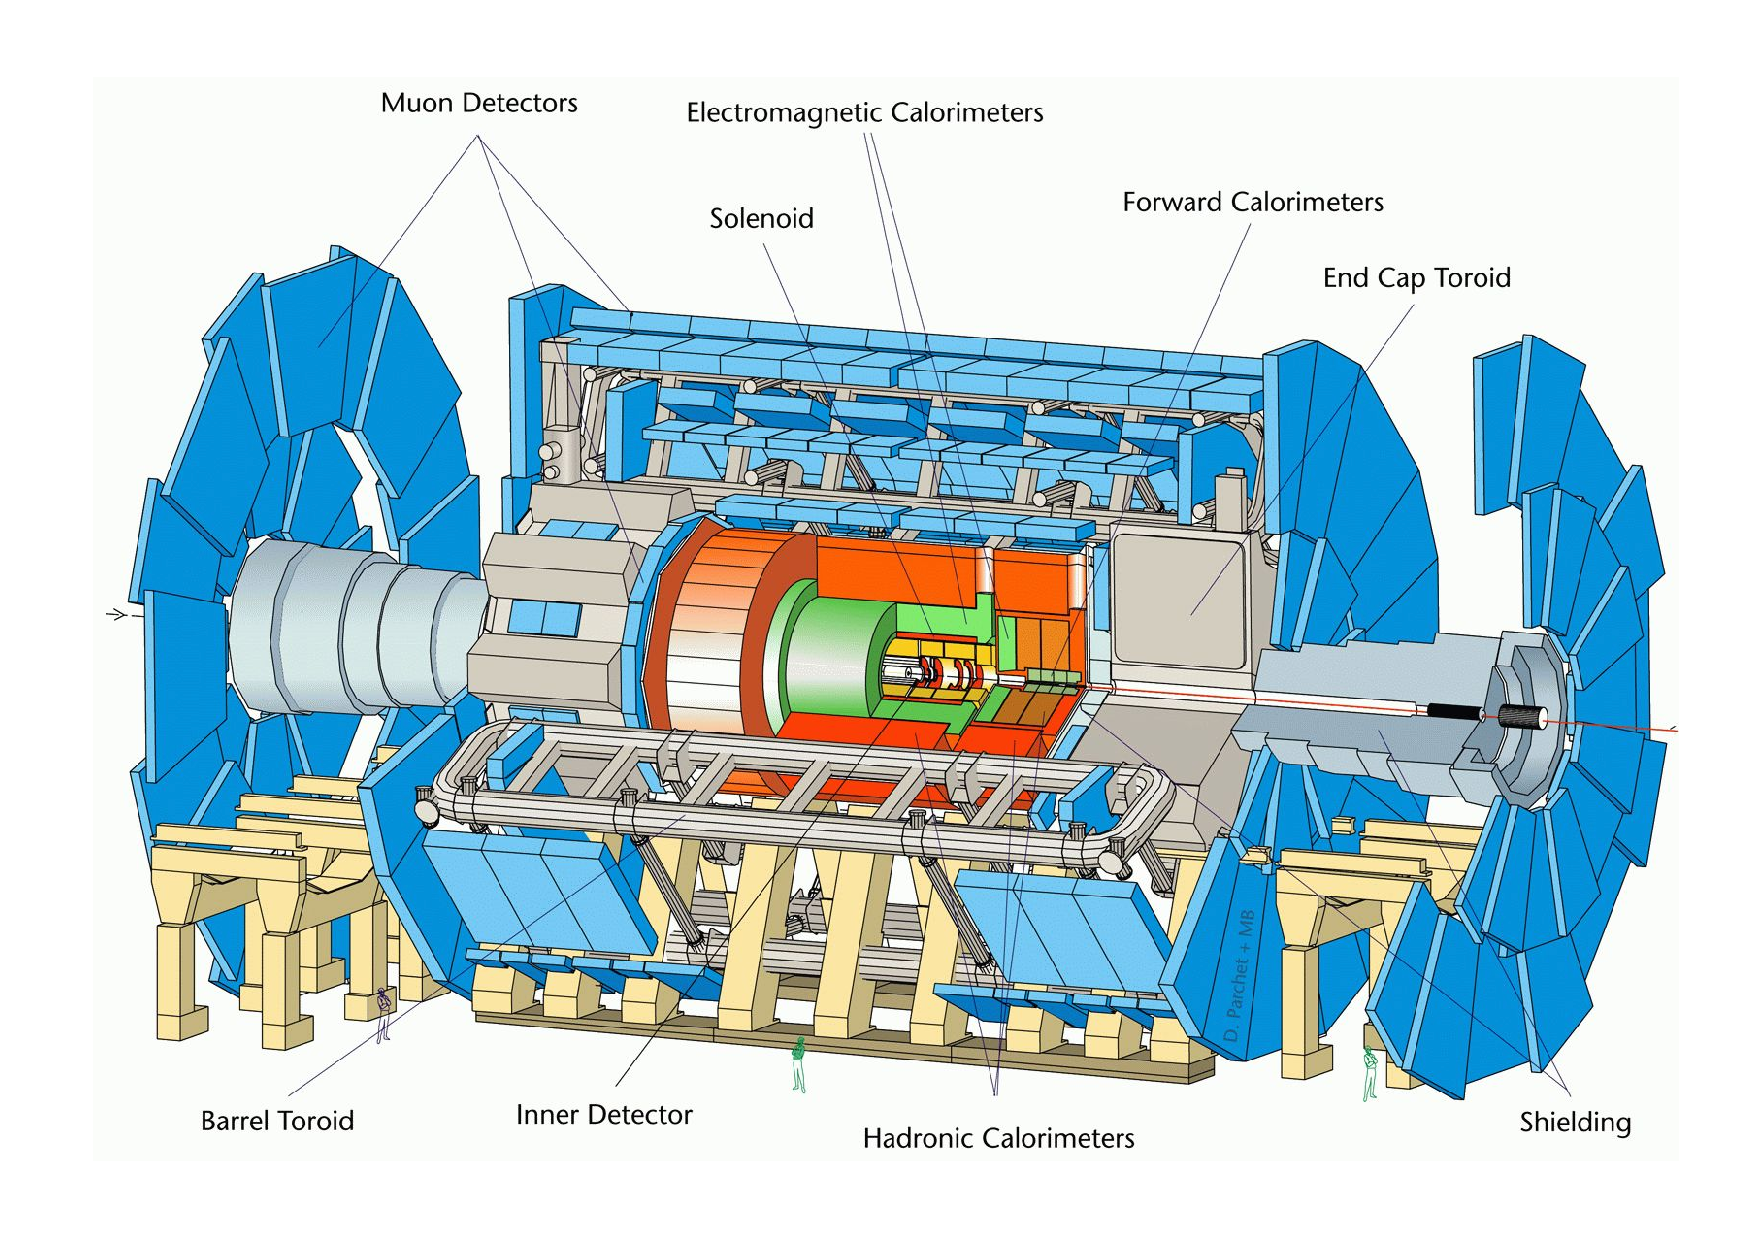
\includegraphics[width=0.7\textwidth]{ATLAS_Diagram.pdf}
    \caption{A diagram that shows the components of the ATLAS detector.}
    \label{ATLAS Detector}
    \end{center}
    \vspace{-0.3cm}
\end{figure}

The ATLAS detector \cite{bib_ATLAS}, shown in Figure \ref{ATLAS Detector},
is a general purpose particle detector which observes collisions of protons accelerated by the LHC. 
The detector is built in many layers around the beam-line where the proton-proton collisions occur;
first the inner detector, which creates tracks showing the trajectories of charged particles, then the EM and hadronic calorimeters, 
which uses particle showers to measure the energy of particles 
and finally the muon detectors which measure the properties of muons.
The solenoid causes a magnetic field throughout the ATLAS detector that causes the trajectories of charged particles to curve,
which aids particle identification and measurements of momentum.  \\

\begin{figure}[!hbt]
  \begin{center}
    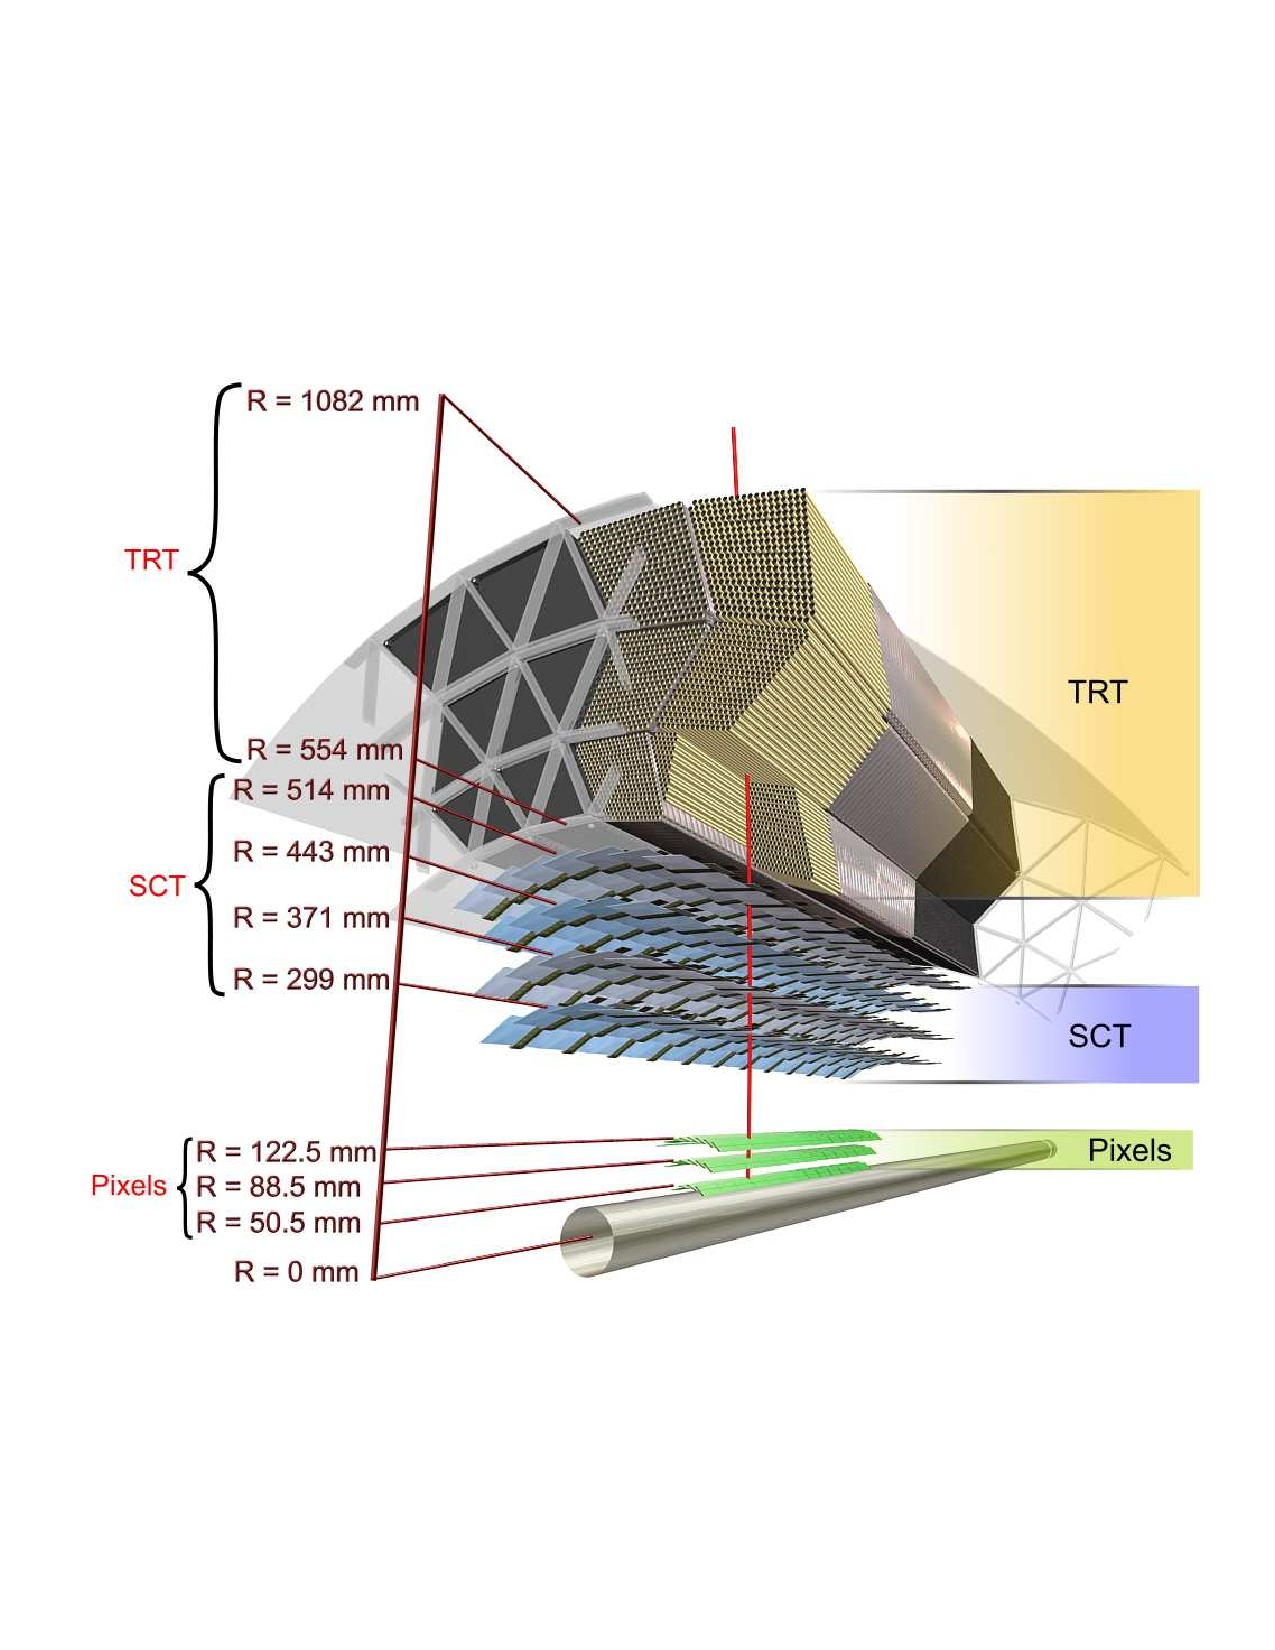
\includegraphics[width=0.55\textwidth]{Inner_Detector.pdf}
    \caption{A diagram that shows the position of the components of the inner detector relative to the beam-line, before the insertion of the IBL. 
      It shows the pixel layers, the silicon layers (SCT) and the straw trackers (TRT). }
    \label{Inner Detector}
    \end{center}
    %\vspace{-1cm}
\end{figure}

The inner detector is the most important part of the detector for flavour tagging \cite{bib_ID}.
The inner detector is made of 4 pixel layers located 33-122.5 mm from the beam-line, 
including the Insertable B-Layer (IBL) \cite{bib_IBL}, a new inner-most silicon layer at 33 mm from the beam-line,
which was inserted into the inner detector in 2014, during the long shutdown between Run-1 and Run-2.
Next is the Semi-Conductor Tracker (SCT), which consists of four layers of silicon microstrip detectors located 299-515 mm from the beam-line. 
The outermost part of the detector is the Transition Radiation Detector (TRT), a section of straw detectors located 554-1082 mm from the beam-line.
Figure \ref{Inner Detector} shows the layout of the inner detector before the insertion of the IBL.
Charged particles leave a small but detectable amount of energy in each layer, which is referred to as a hit. 
The pattern of hits in the layers is then analysed to reconstruct tracks that represent the trajectories of particles as they pass through the layers.
The reconstructed tracks are then used to search for particles that come from an offset vertex. \\

In Run-2, the ATLAS experiment has been taking data at a rate of 40 MHz. However, it is impossible to write and store data that is taken at this rate.
The ATLAS experiment uses a trigger system to reduce the event rate by selecting the events of interest that contain 
high-$p_{T}$\footnote{$p_{T}$ refers to the component of momentum transverse to the beam-line.} 
physics objects, which 
indicate that a hard scatter has occurred in that event. 
The ATLAS trigger-system has two levels; the first level is hardware based and reduces the rate from 40 MHz to 100 kHz.
The first level then seeds a software 
based trigger level, the higher-level trigger (HLT), which then further reduces the event rate to 1 kHz \cite{bib_trigger}. 

\newpage
\section{Flavour Tagging Algorithms}  \label{s_Algos}

There are three main base flavour tagging algorithms used at ATLAS \cite{bib_algos}, each of which utilise the extended lifetimes of the heavy hadrons by searching for tracks,
reconstructed in the inner detector, that show that there are particles coming from a decay offset from the primary vertex.
The three base algorithms are then combined to create a multivariate tagger, which has the optimal flavour tagging performance.
Figure \ref{B-Tagging_Diagram} illustrates the key features of the three algorithms.

\begin{figure}[!htb]
  \begin{center}
    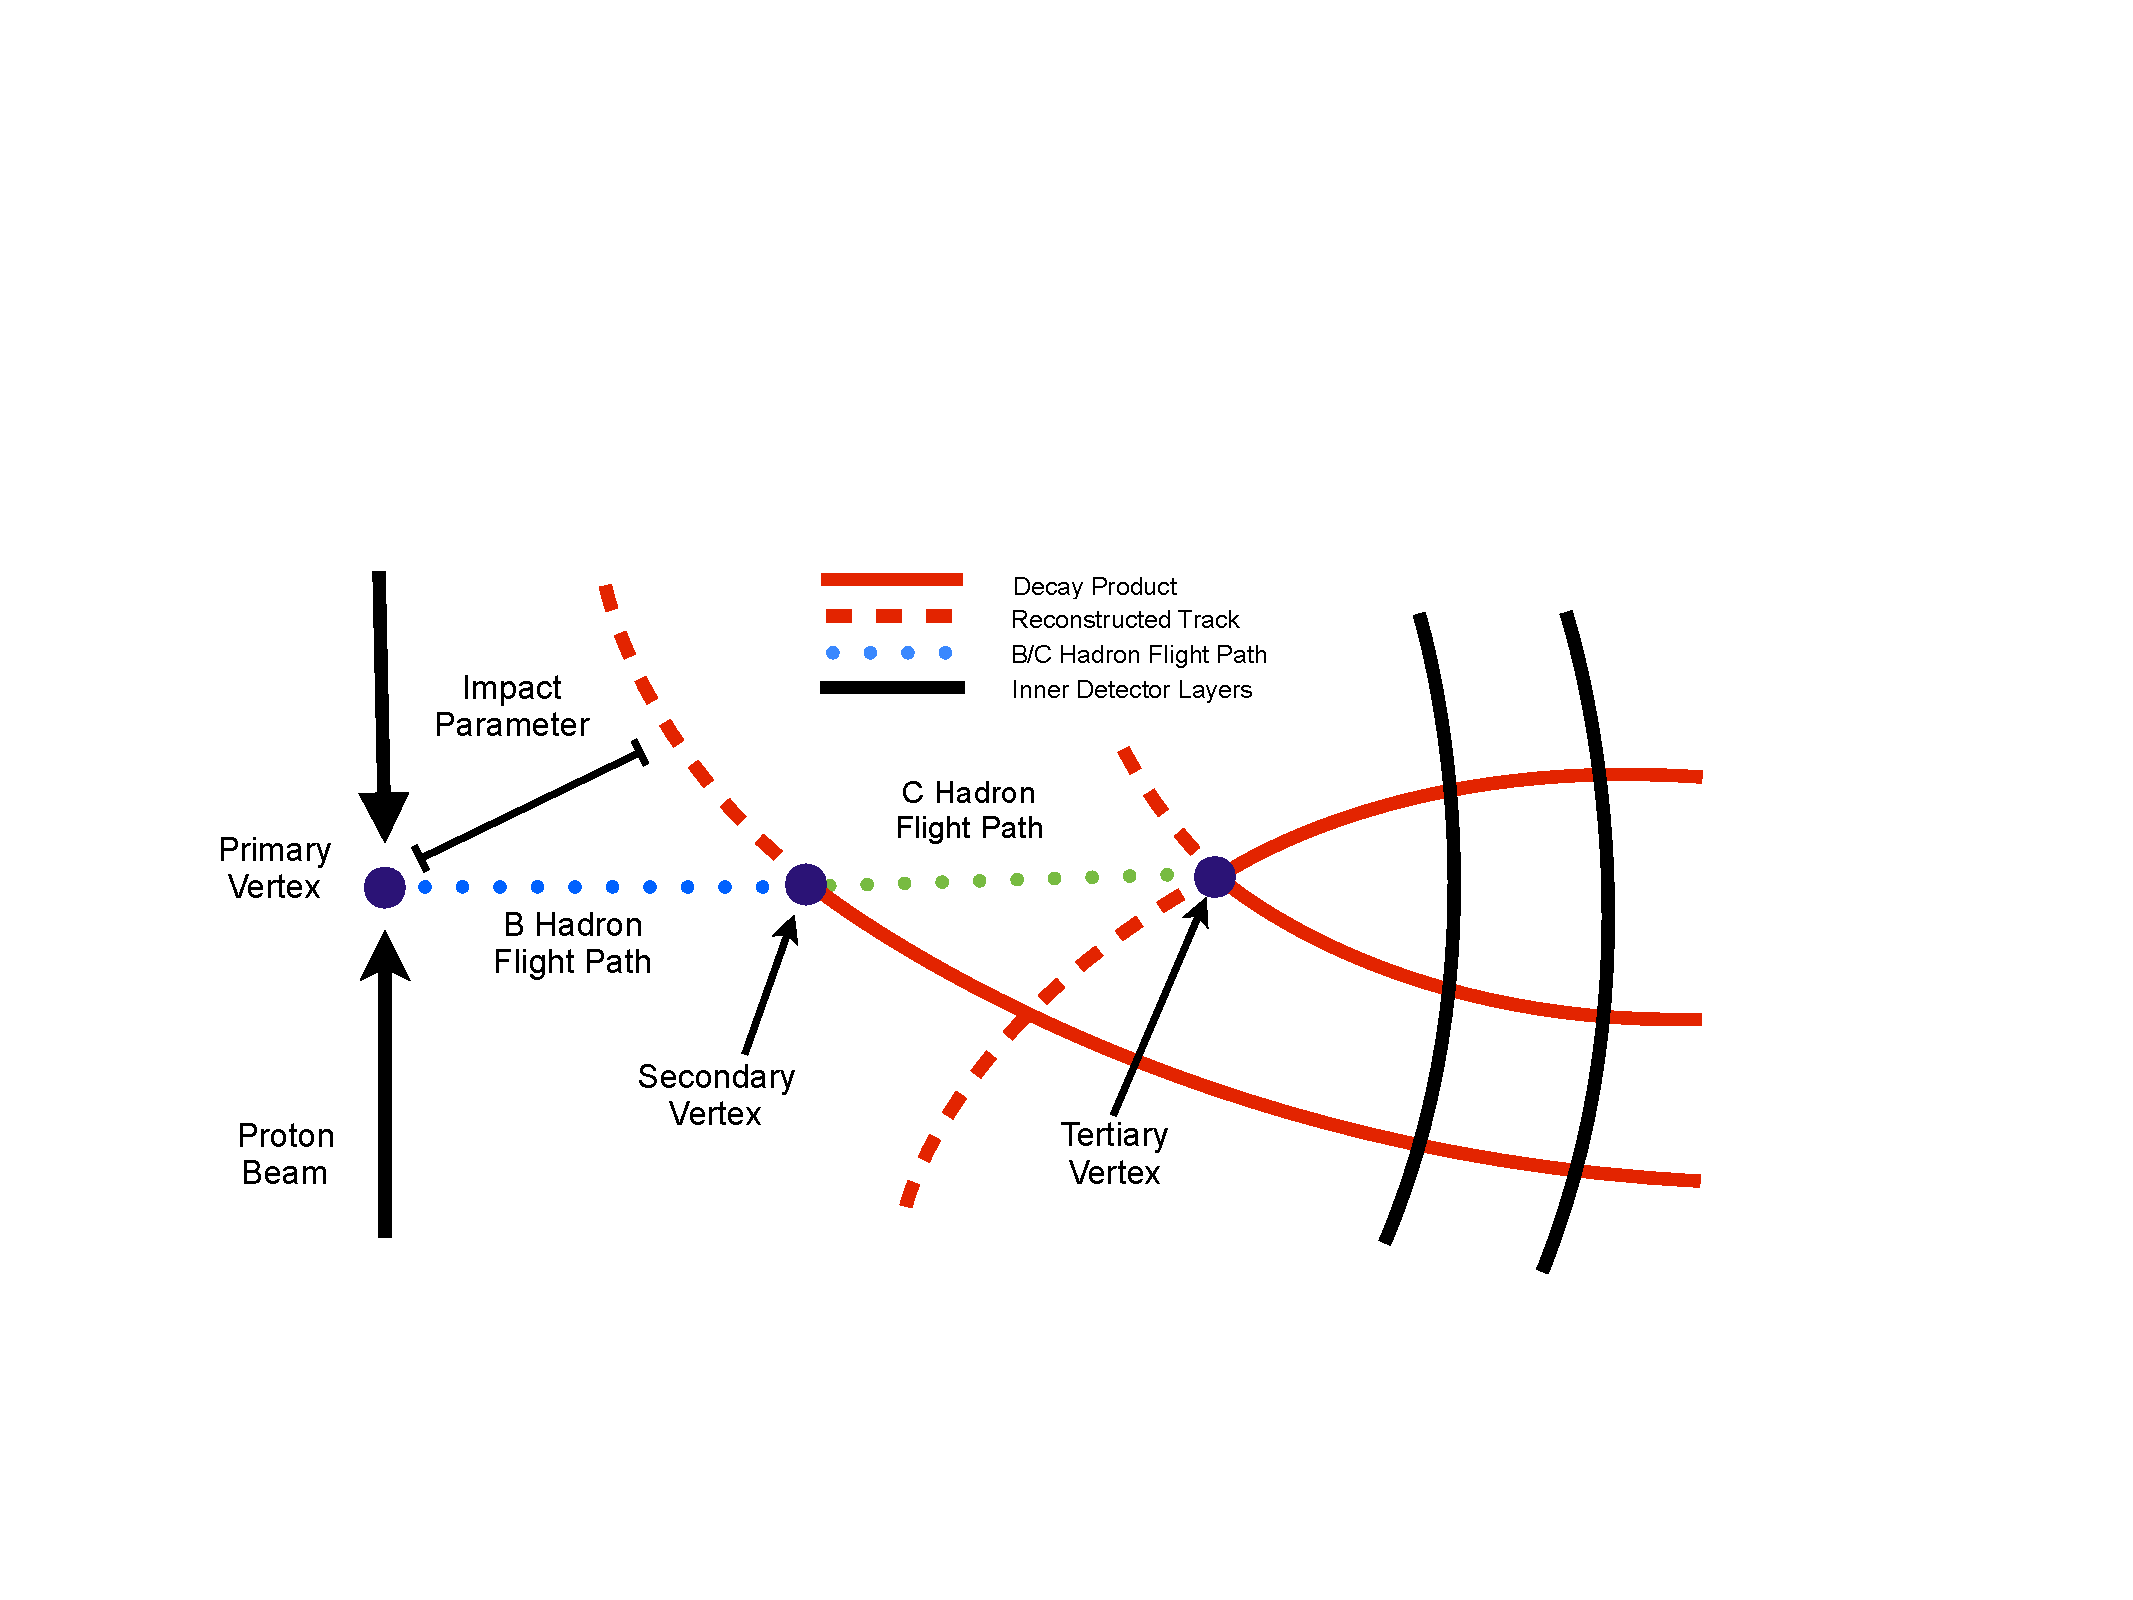
\includegraphics[width=0.7\textwidth]{B-Tagging_Diagram.pdf}
    \caption{A diagram to illustrate the key features in a \textit{b}-jet that are used by the base flavour tagging algorithms.}
    \label{B-Tagging_Diagram}
  \end{center}
  \vspace{-0.5cm}
\end{figure}

\subsection{Impact Parameter Based: IPxD}  \label{ss_Algos_IPxD}

The IP3D algorithm is an impact parameter based flavour tagging tool. 
A track corresponding to a particle coming from the offset decay vertex in a \textit{b}- or \textit{c}-jet is likely to have a large distance of 
closest approach to the primary vertex, known as the impact parameter, meaning that the distribution of track impact parameter is different for each of the jet-flavours.
In this algorithm, for all tracks associated to a jet, the impact parameter is calculated in both the transverse (perpendicular to beam-line)
and longitudinal (parallel to beam-line) direction, which are referred to as $d_{0}$ and $z_{0}$.
Then the IP3D algorithm calculates a likelihood of the jet having a specific flavour, 
based on the distributions of the impact parameters ($d_{0}$, $z_{0}$), and the distributions of their significances 
($d_{0}/\sigma _{d0}$ and  $z_{0}/\sigma_{z0}$) of tracks inside the jet. 
Another similar algorithm, IP2D, also calculates the jet flavour likelihood from just the transverse distributions, ($d_{0}$ and $d_{0}$ significance), which is more
robust to pile-up, as tracks from pile-up jets are likely to have a large $z_{0}$ significance value.

\subsection{Secondary Vertex: SV1}  \label{ss_Algos_SV1}

The SV1 algorithm aims to reconstruct a secondary vertex of two or more intersecting tracks, corresponding to the decay of a heavy-flavour hadron. 
Properties of the reconstructed secondary vertex that show flavour discrimination are, for example; the vertex 
invariant mass and energy fraction (fraction of jet energy contained in the secondary vertex) which will be large for 
\textit{b}-jets due to the heavy mass of the \textit{b}-hadron 
\footnote{Mass of a B-meson $\sim$ 5 GeV and the mass of a D-meson $\sim$ 1.9 GeV, which are the most common heavy hadrons in a \textit{b}- and \textit{c}-jet respectively.}, 
the distance in the transverse plane between the 
primary vertex and the secondary vertex (2D flight path $L_{XY}$), which will be large for \textit{b}-jets due to the long lifetime of the \textit{b}-hadron,
and the number of tracks at the secondary vertex, which will be large for well constructed secondary vertices, which are more likely in \textit{b}-jets.


\subsection{Multi-Vertex: JetFitter}  \label{ss_Algos_JF}

The JetFitter algorithm (JF) attempts to reconstruct the full decay chain of the \textit{b}-hadron into a charmed-hadron and then into light-hadrons. 
This is done by assuming that all vertices lie on a common \textit{b}-flight axis, and then constructing vertices from the intersection of
one or more tracks and the flight axis.
Reconstructed secondary and tertiary vertices correspond to the decays of the \textit{b}-hadron and charmed-hadron, as seen in Figure \ref{B-Tagging_Diagram}.
Discriminating variables of JF, similarly to SV1, are vertex mass, energy fraction, number of vertices with two or more tracks and number of one track vertices.

\subsection{Multivariate Algorithms: MV2}  \label{ss_Algos_MV2}

The three base algorithms are combined in a boosted decision tree (BDT), which is a machine-learning technique for combining the many flavour-discriminating variables.
As shown in Figure \ref{MV2_Diagram}, MV2 combines the likelihood output of IP3D and IP2D, with the discriminating variables of SV1 and JF discussed above.
This is in contrast to the previous multivariate tagger used in Run-1, MV1, which inputted
the likelihood of a jet having a certain flavour from each of the three base algorithms separately.
For Run-2 the recommended \textit{b}-tagging tool is MV2c20 which has been trained on a sample containing 20\% charm, to give strong light- and \textit{c}-rejection rates.
 
\begin{figure}[!htb]
  \begin{center}
    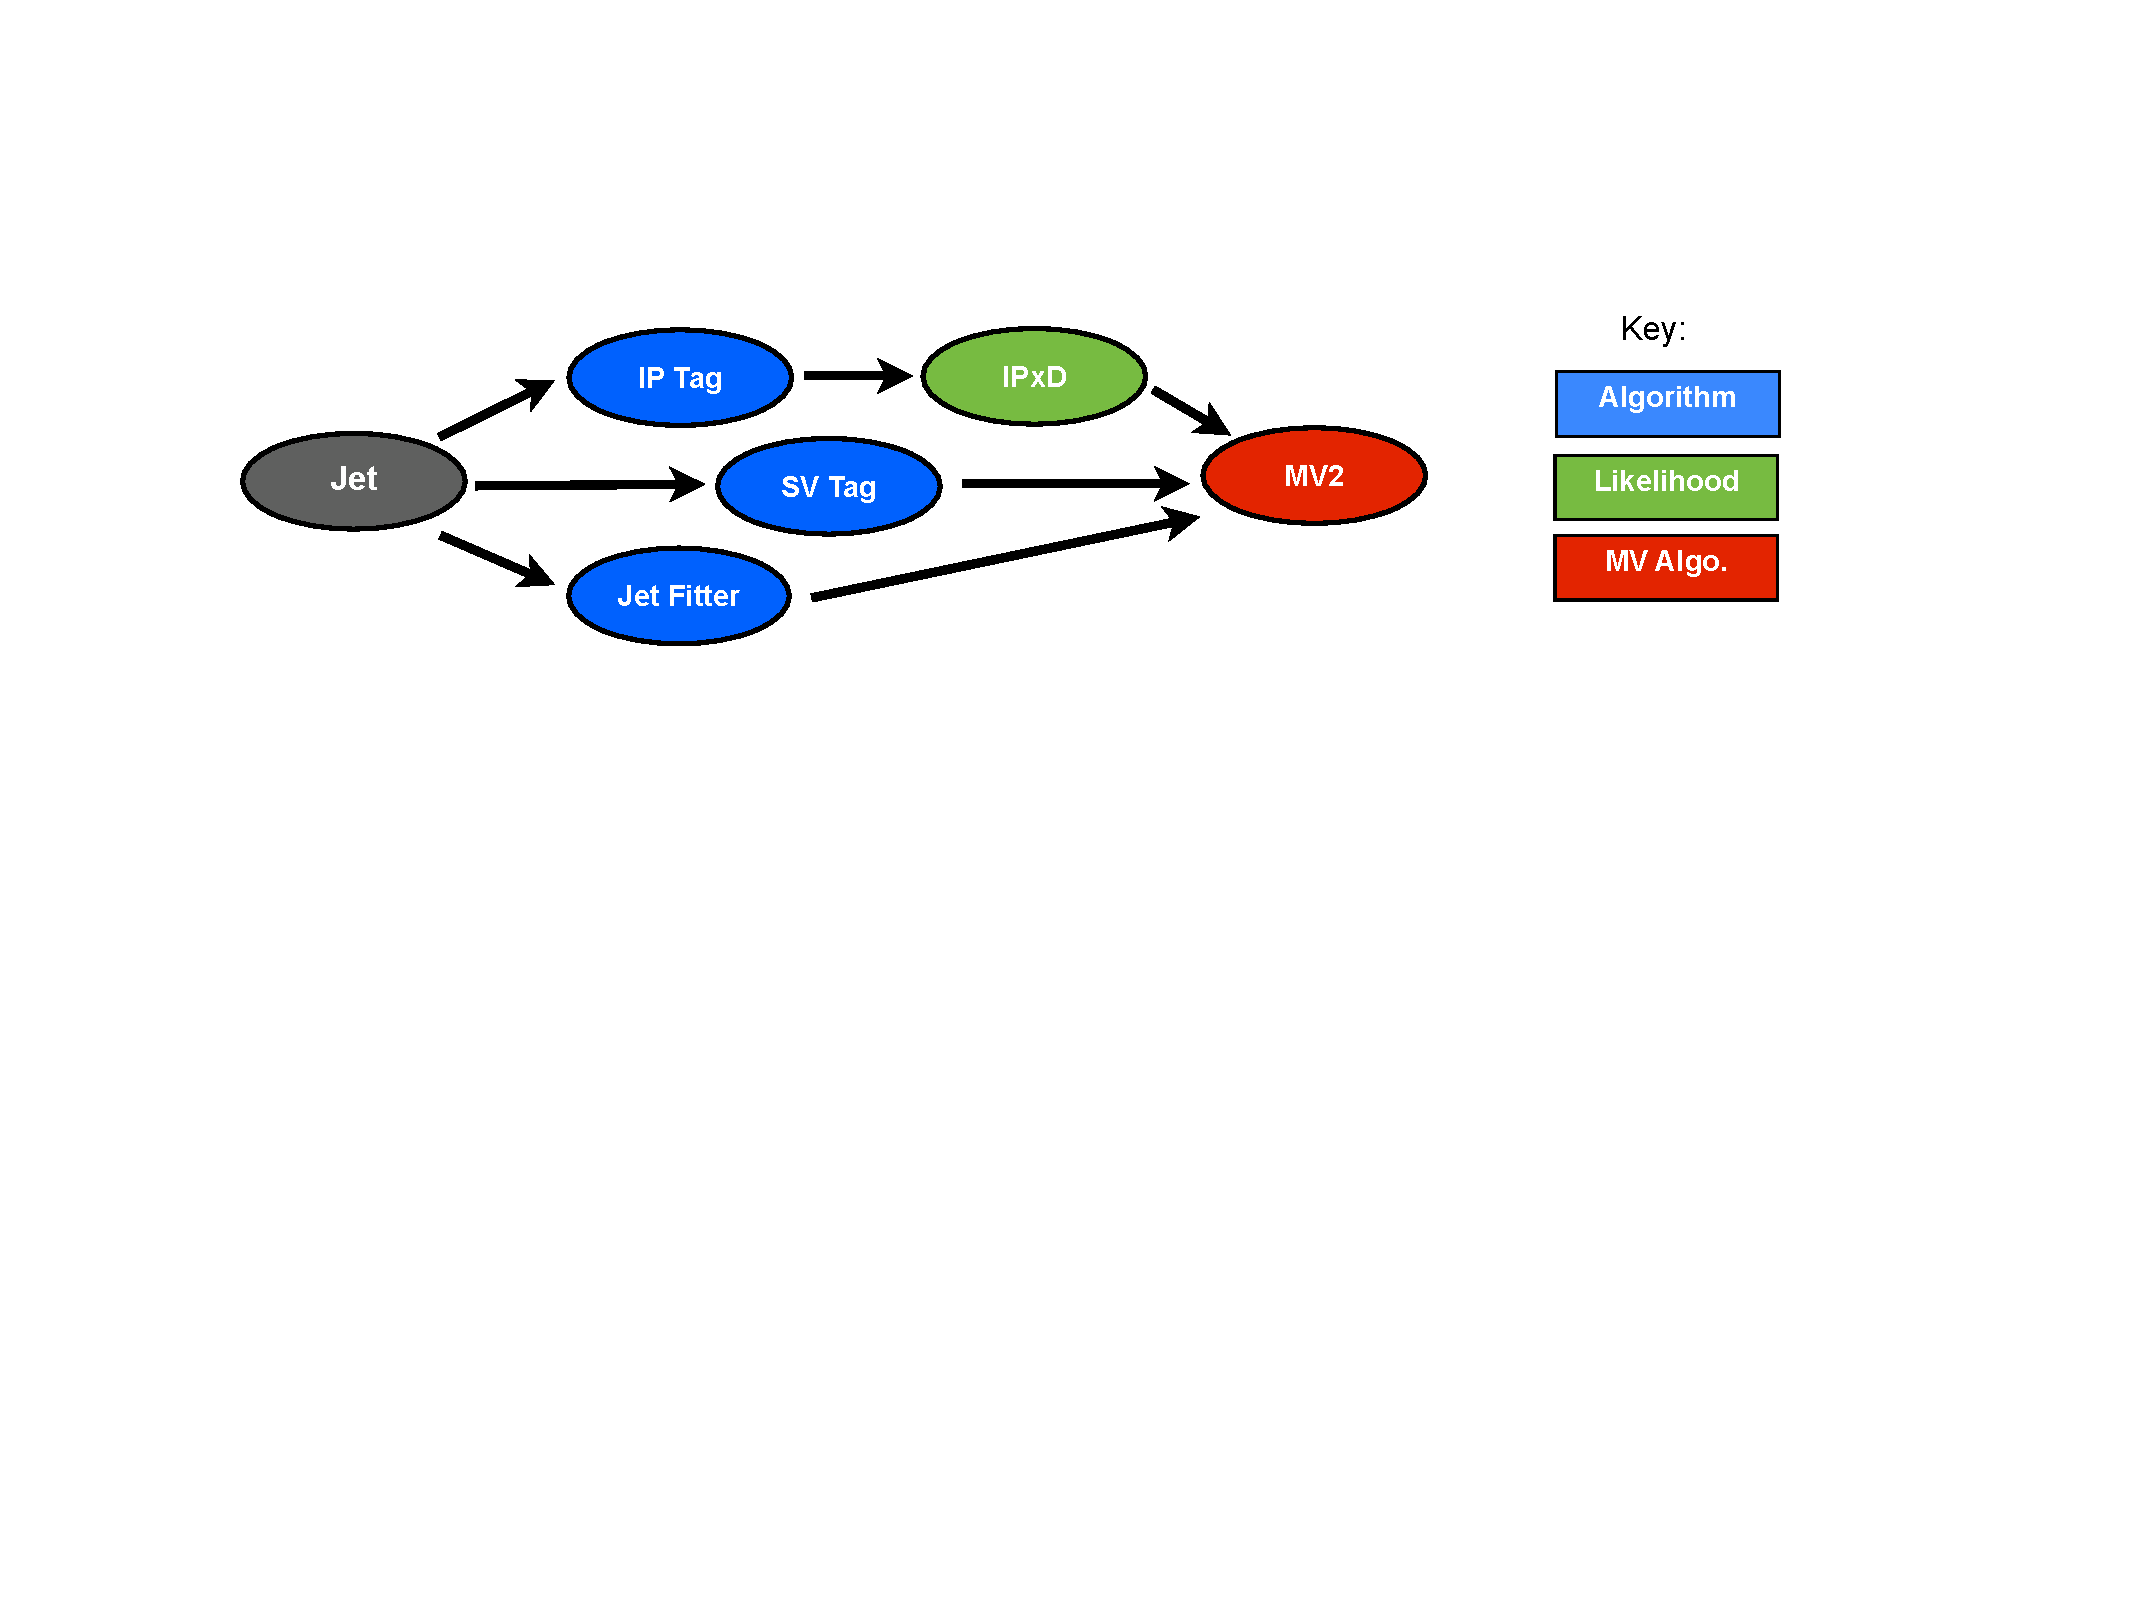
\includegraphics[width=0.8\textwidth]{MV2_h.pdf}
    \caption{A diagram to show the how the three base flavour tagging algorithms are combined in the MV2 algorithm.}
    \label{MV2_Diagram}
  \end{center}
  \vspace{-1cm}
\end{figure}

\section{Data Commissioning in Run-2} \label{s_comm}

During the long shutdown between Run-1 and Run-2 there have been many changes that affect
 flavour tagging performance;
improved and optimised base algorithms, the change from MV1 to MV2, and the addition of the IBL.
The understanding of the performance of flavour tagging after these changes is validated in data  
by comparing the key variables relevant to flavour tagging in data and simulation. 
This study focuses on comparing data to simulation in events from an inclusive dijet sample.
A similar study has been done in $t\bar{t}$ events \cite{bib_ttbar_comm}.

\subsection{Data Samples} 

\subsubsection{Experimental data sample}

The experimental data sample used 56 pb\textsuperscript{-1} of proton-proton collisions at $\sqrt{s}$ = 13 TeV collected by the ATLAS detector from May to July 2015.
Data was only used if it was collected when beam conditions were stable and the inner detector and calorimeter detectors were fully functional.

\subsubsection{Simulated sample} \label{ss_comm_simulation}

The experimental data sample is being compared to a sample of simulated QCD multi-jet events.
The events are simulated by a Monte Carlo generator, PYTHIA 8 \cite{bib_pythia8}, 
applied with the A14 \cite{bib_A14} underlying event tune and the NNPDF23LO \cite{bib_PDF} parton density function set (PDF).
The decays of \textit{b}-hadrons are generated using the EVTGEN \cite{bib_evtgen} decay package, which uses experimental data to correct the Monte Carlo generation.
Pile-up is simulated by adding to the event minimum bias events generated by PYTHIA 8.
Then the response of the ATLAS detector to the generated events is simulated using a full model of the ATLAS detector \cite{bib_atlas-simulation},
built using GEANT4 \cite{bib_geant4} to simulate the interactions between the generated particles and the detector material.
The simulation is then normalised to the number of events in the data sample, after event selection, described in Section \ref{ss_comm_event}, has been applied to both samples.

\subsection{Object and Event Selection} \label{ss_comm_event}

The primary vertex, the point where the hard-scatter occurred, is reconstructed by looking for multiple tracks from the inner detector that intersect the beam-line at the same point.
In the case that there are several candidate vertices, the vertex with the highest sum of track $p_{T}^2$ is used. \\

Jets are reconstructed with the anti-$k_{t}$ algorithm \cite{bib_AKT},
which selectively merges pairs of energy clusters in the calorimeter depending on the pairs' transverse momenta and 
$\Delta R$ \footnote{$\Delta R = \sqrt{(\Delta \phi)^2+(\Delta \eta)^2}$} separation to create the jet. 
The radius parameter for the anti-$k_{t}$ algorithm, which defines the maximum $\Delta R$ separation that can be merged, is 0.4. 
The clusters are calibrated on the EM-scale, meaning that they are calibrated using the assumption that all interactions between the detected particle and the detector are
through the EM-force, as it would be for a lepton or a photon.
However, for hadronic jets the dominant interaction between the jet and the detector is the strong-interaction with a smaller contribution from the EM-interaction,
the combination is known as the hadronic-scale.
To obtain the hadronic-scale, a $p_{T}$ and $\eta$ \footnote{\vspace{0.5mm}  $\eta = -\ln\left[\tan(\frac\theta{2})\right]$}
dependant correction factor is applied to the jets, which has been derived from Monte Carlo simulations.
A preliminary version of the jet energy scale calibration is applied, which corrects from simulated detector measurements to the detector measurements observed in data.
The jet energy scale calibration is derived using an in-situ jet calibration that considers momentum balance 
in events that contain only a Z-boson and a jet in the final state \cite{bib_JES}. 
If corrections from the EM-scale to the hadronic-scale and the jet energy scale calibration are not applied,
then an incorrect measurement of the jet-$p_{T}$ will be made, which is significant as flavour-tagging performance is strongly-correlated to jet-$p_{T}$.\\

At ATLAS, due to the high number of particles in each beam, there can be multiple proton collisions per beam crossing,
meaning that there are many particles that come from vertices other than the primary vertex, known as pile-up.
Pile-up can cause problems with measurements of jets at ATLAS; 
specifically pile-up can cause additional tracks in the inner detector which can be falsely associated to a jet which affects flavour tagging performance 
and pile-up can also be included in the energy clusters in the calorimeter causing jet-$p_T$ to be mismeasured.
To reduce the contribution of pile-up, a new algorithm, the jet vertex tagger (JVT)\cite{bib_JVT}, is used. 
JVT is a multivariate algorithm that combines two variables; the first related to the fraction of tracks coming from the primary vertex, the second is the ratio of the sum of 
$p_{T}$ for tracks associated to the jet to jet-$p_{T}$. The JVT algorithm returns an output between -0.1 and 1, a larger JVT output indicating that the jet is less likely to be pile-up.
We require that jets have $p_{T} >$ 35 GeV, $|\eta| <$ 2.4 and JVT output $>$ 0.641 if jet-$p_{T} <$ 50 GeV. \\

As discussed in Section \ref{s_ATLAS}, a two level trigger system is used at ATLAS to select events, 
which means each event has to pass first a Level 1 (L1) trigger which removes events based on coarse information, 
and then this L1 trigger feeds a Higher-Level Trigger (HLT), which removes further events with the full-event information.
Events are selected if they have fired the HLT\_j60 trigger, a higher level trigger that selects events if there is a jet with $p_{T} >$ 60 GeV, 
which is fed by the L1\_J20 trigger, a level 1 trigger that selects events if there is $\Sigma p_{T} >$ 20 GeV deposited in a 0.8 x 0.8 $\eta-\phi$ region of the calorimeter.
It is required that the leading jet \footnote{ The leading jet is the jet with the highest $p_T$ in that event, and the subleading jet is the jet 
with jet with the second highest $p_T$ within that event.}
has $p_{T} >$ 70 GeV, such that we are in a kinematic region where trigger efficiency is optimal.
A further cut is applied to the simulation sample requiring that the mean $p_{T}$ of the leading and subleading jet is less than 1.4 times the truth $p_{T}$ of the 
leading jet; this cut is used to prevent tails in the jet-$p_T$ distribution causing a non-smooth overall jet-$p_T$ spectrum.  \\

In simulation, we assign flavour to jets by matching truth-level heavy-hadrons with $p_{T} >$ 5 GeV and $\Delta R <$ 0.3 between the hadron and the jet.
If a \textit{b}-hadron is matched to a jet, the jet is then declared a \textit{b}-jet; this process is then repeated for \textit{c}-hadrons and then $\tau$ leptons.
If no match between \textit{b}, \textit{c} or $\tau$ is achieved then the jet is assigned as a light-flavour jet.
   
\subsection{Reweighting Simulation}

When the simulation sample is created, the exact beam conditions of the data sample that we will compare to is not known.
One of the parameters that is related to the beam conditions is the average number of interactions per beam crossing, $< \mu >$.
The value of $< \mu >$ is related to the amount of pile-up in an event, and as discussed in Section \ref{ss_comm_event}, 
pile-up can influence flavour tagging performance,
thus, to be able to compare flavour-tagging performance in simulation and data the $< \mu >$ must be the same.
Initially, the simulation sample is produced with a broad $< \mu >$ distribution and
then the $< \mu >$ distribution of the simulation is reweighted such that it is identical to the experimental data set.

%Figure \ref{avgmu} compares the $< \mu >$  distributions of the simulation sample and the data sample,
%both before and after reweighting of the simulation sample.
%Also shown is a ratio plot of data to simulation.

%\begin{figure}[!htb]
%	 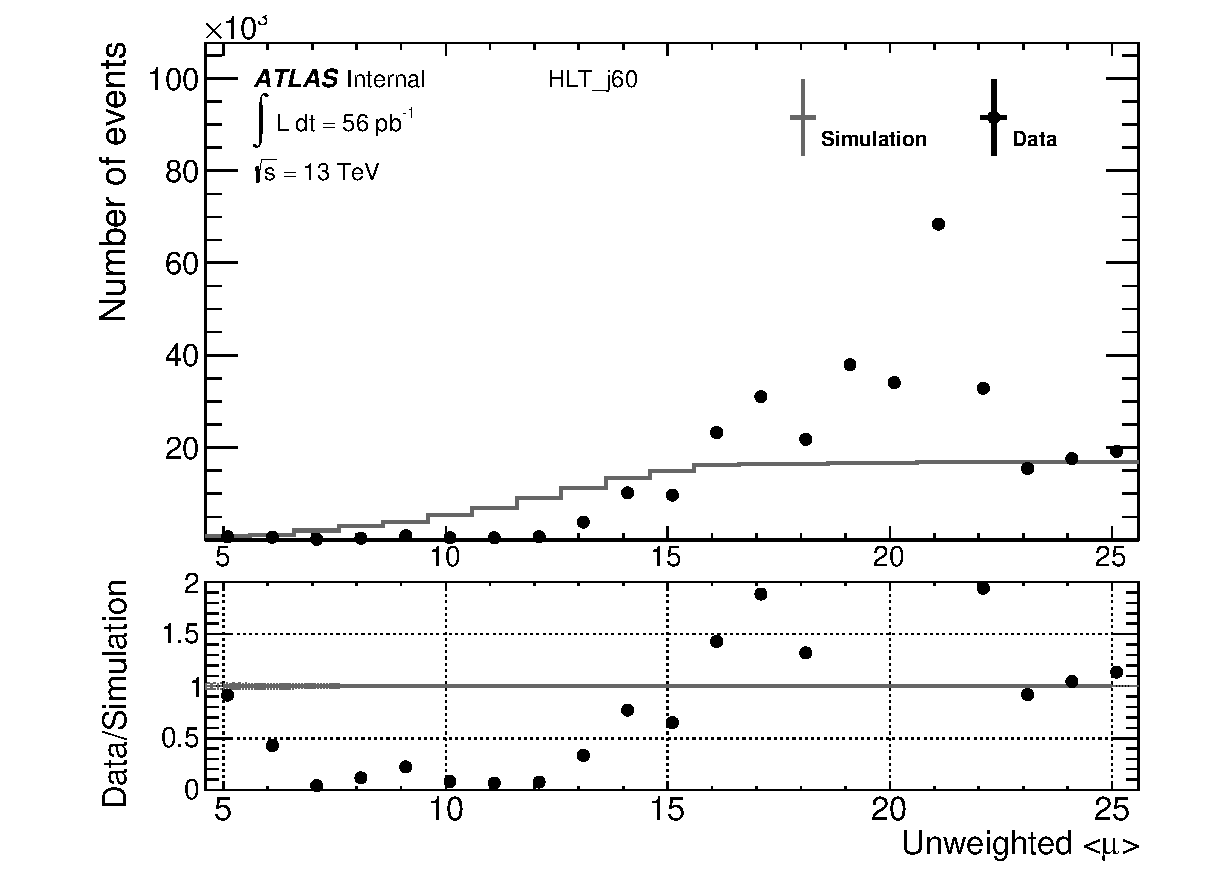
\includegraphics[width=0.45\textwidth]{plots/Event/avgmu_norw.eps}
%	 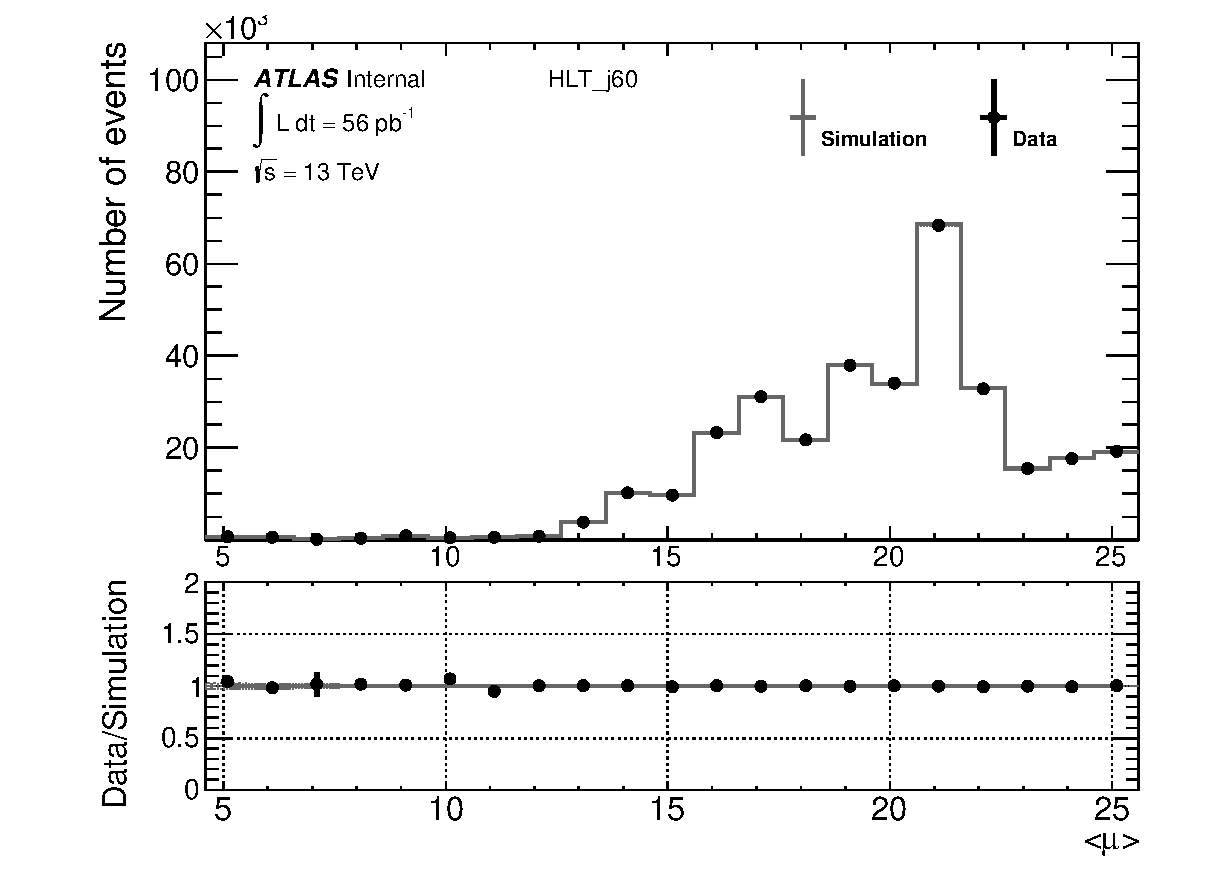
\includegraphics[width=0.45\textwidth]{plots/Event/avgmu.eps}
%	 \caption{The average number of pile-up interactions, $<\mu >$, for data (solid points) and simulation (grey shaded), before and after reweighting.}
%        \label{avgmu}
%  \vspace{-0.5cm}
%\end{figure}

\subsection{Jet Kinematics}


%\begin{figure}[!htb]
%	 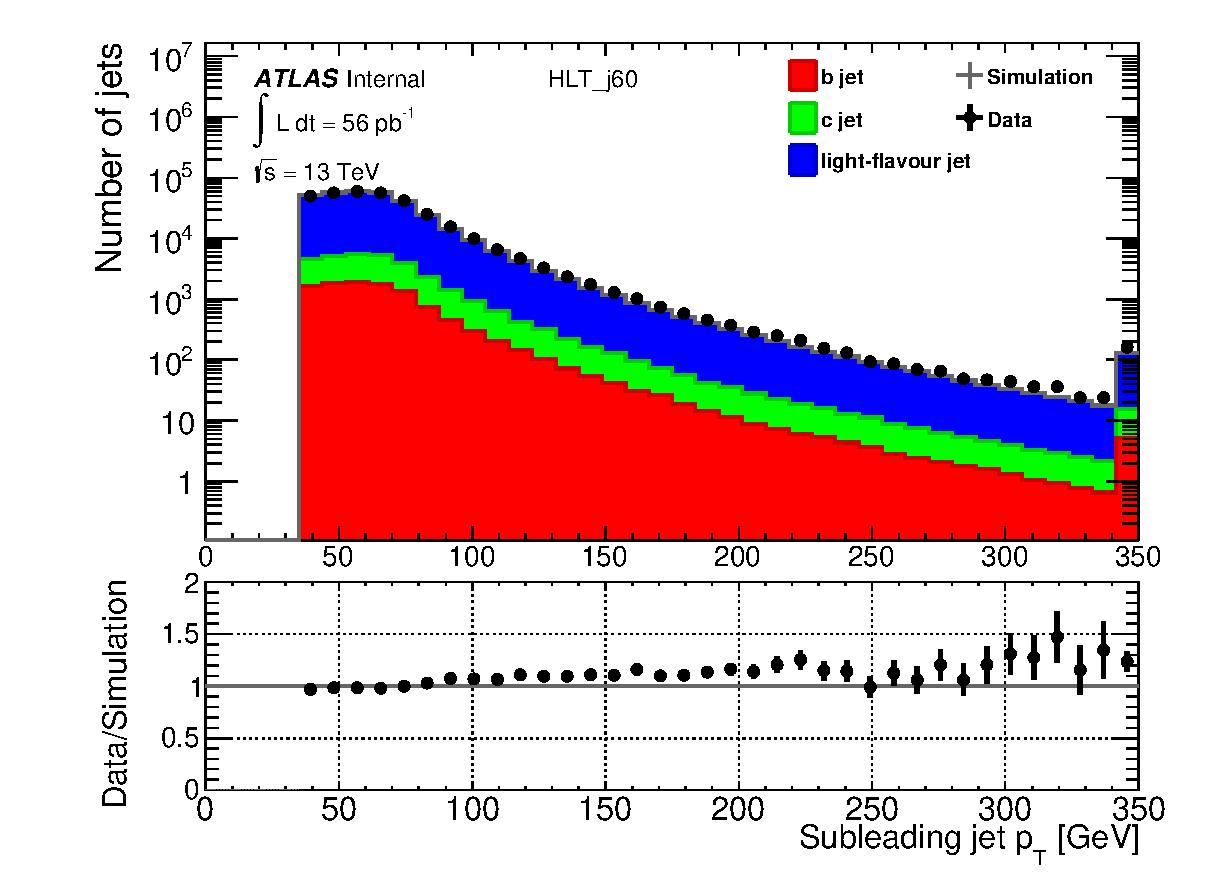
\includegraphics[width=0.45\textwidth]{plots/SubLeadingJet/jetPt_sublead.eps}
%	 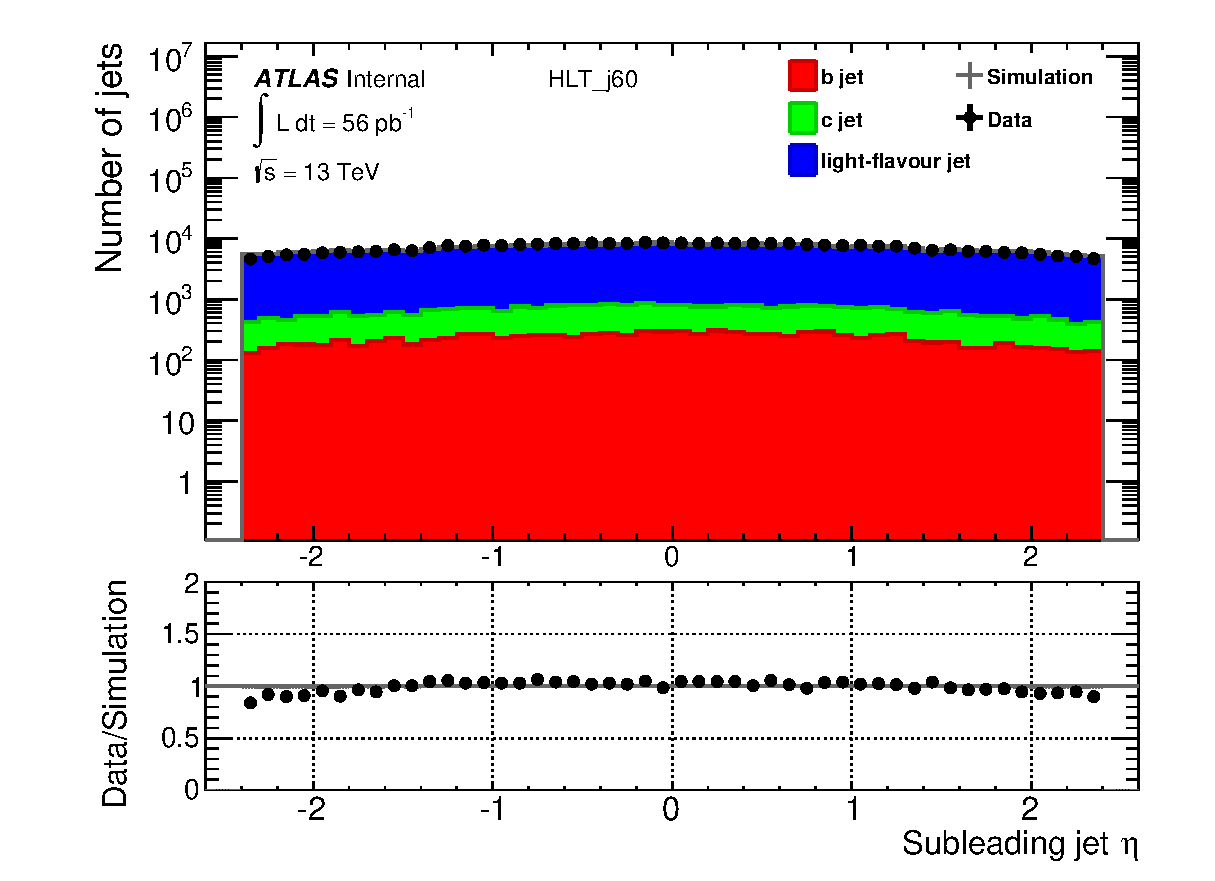
\includegraphics[width=0.45\textwidth]{plots/SubLeadingJet/eta_sublead.eps}
%	 \caption{Distributions of $p_{T}$ (left) and $\eta$ (right) for the subleading jet, for data (solid points) and simulation (grey shaded); 
%           which is shown as a stack of its flavour components; \textit{b}, \textit{c} and light flavoured jets (red, green and blue respectively).}
%         \label{SubLeadJetKine}
  %\vspace{-1cm}
%\end{figure}

Flavour tagging performance is sensitive to the kinematics of the jet; in particular jet-$p_{T}$ and pseudorapidity ($\eta$).
%and number of associated tracks.
Hence it is important that before examining flavour tagging directly that it is demonstrated that the key jet kinematics in data are well modelled
in simulation.
%In addition demonstrating that the JVT distribution is well modelled shows that the contribution from pile-up is well understood. 
In Figure \ref{LeadJetKine} the jet-$p_T$ and $\eta$ distributions for the leading jet are compared for data and simulation.
The simulation is shown as a stacked histogram of its flavour components, with red for b-jets, green for c-jets and blue for light flavoured jets.
Data is represented by solid points and simulation is shown by a grey line.
%In Figure \ref{SubLeadJetKine}, the jet-$p_{T}$ and $\eta$ distributions for the subleading jet are shown.
The simulation shows good agreement with the data.

\begin{figure}[!htb]
	 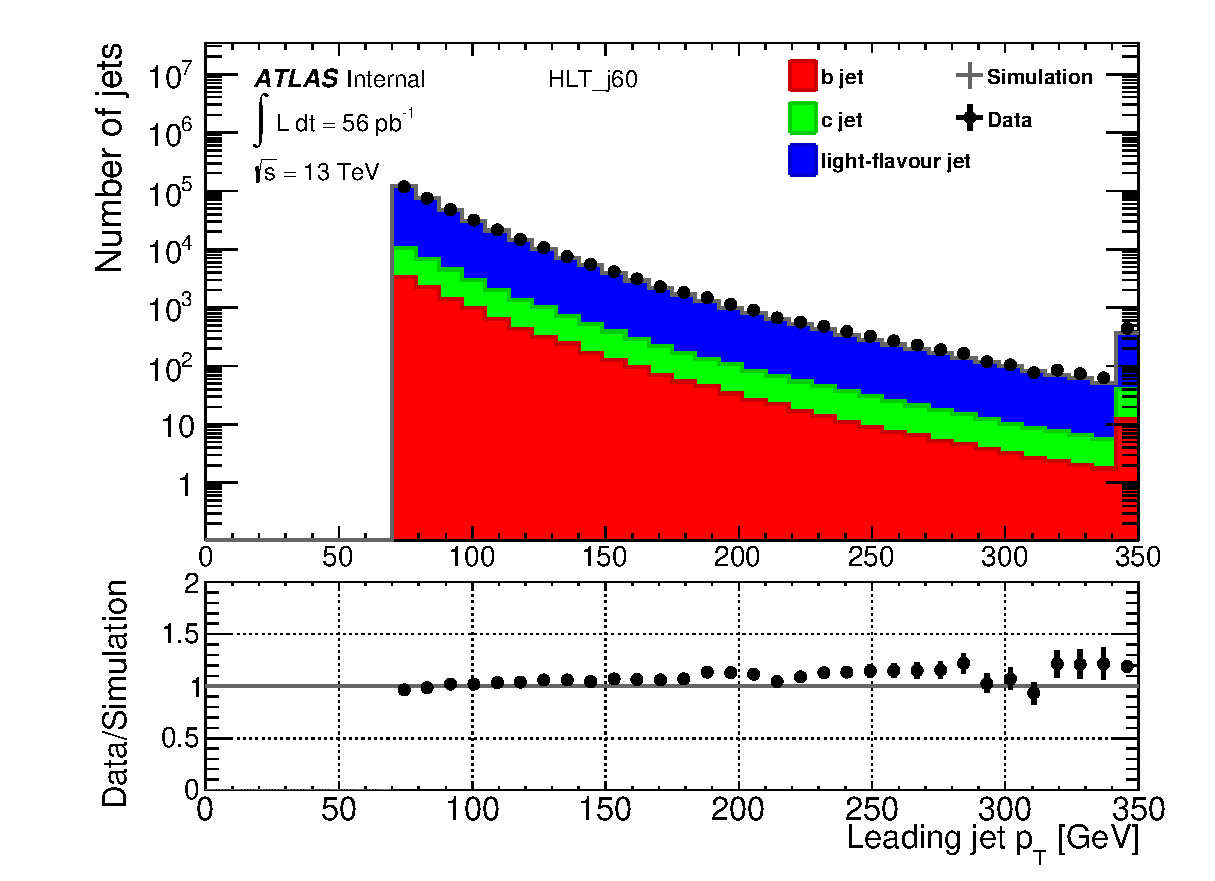
\includegraphics[width=0.45\textwidth]{plots/LeadingJet/jetPt.eps}
	 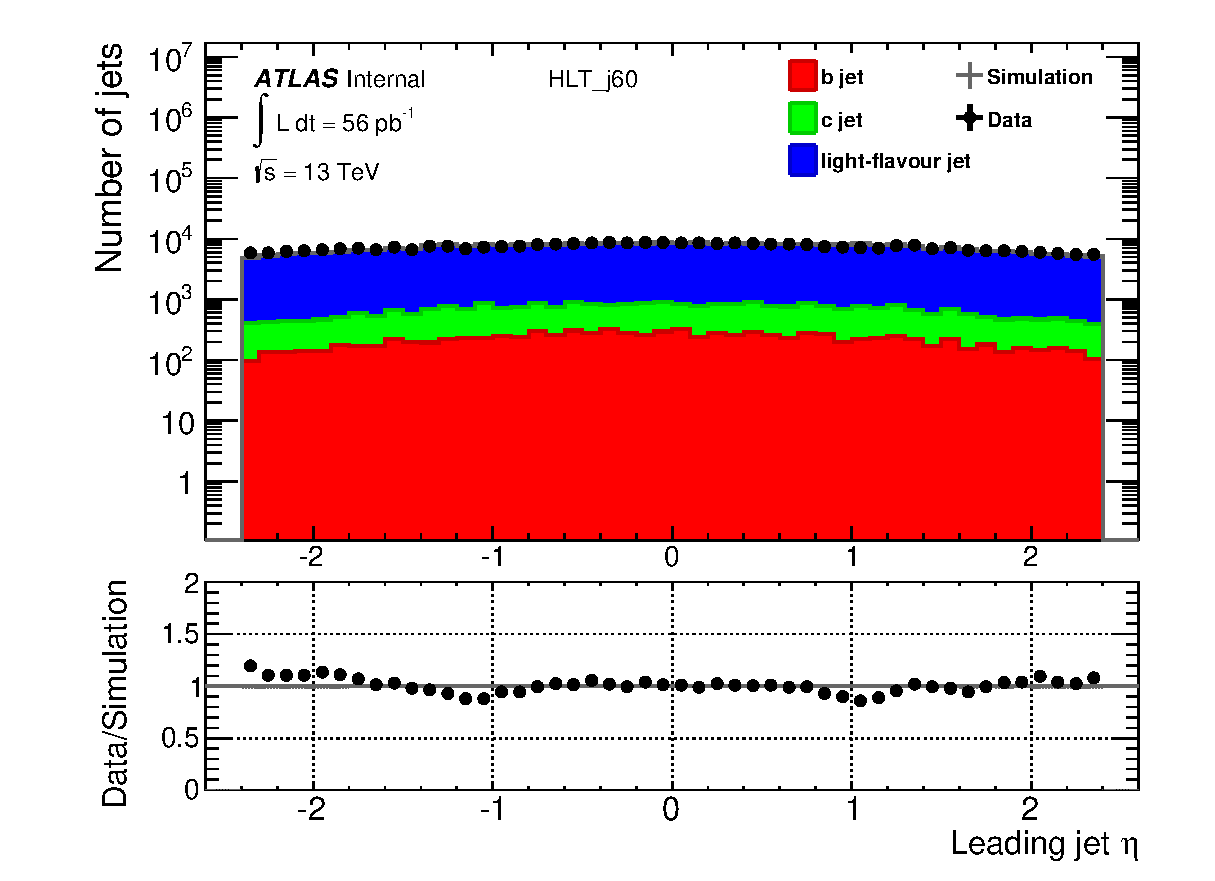
\includegraphics[width=0.45\textwidth]{plots/LeadingJet/eta.eps}
	 %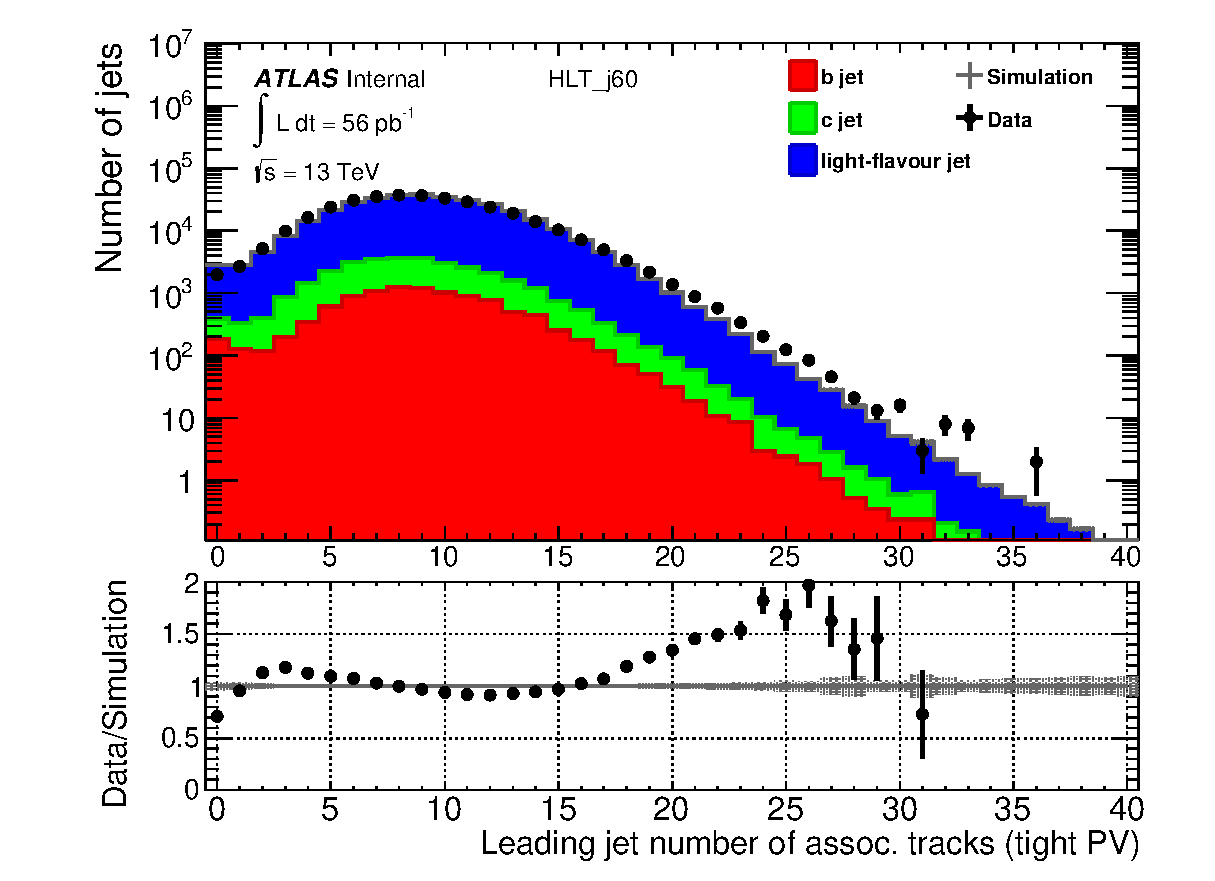
\includegraphics[width=0.45\textwidth]{plots/LeadingJet/sumtrk_ntrk.eps}
	 %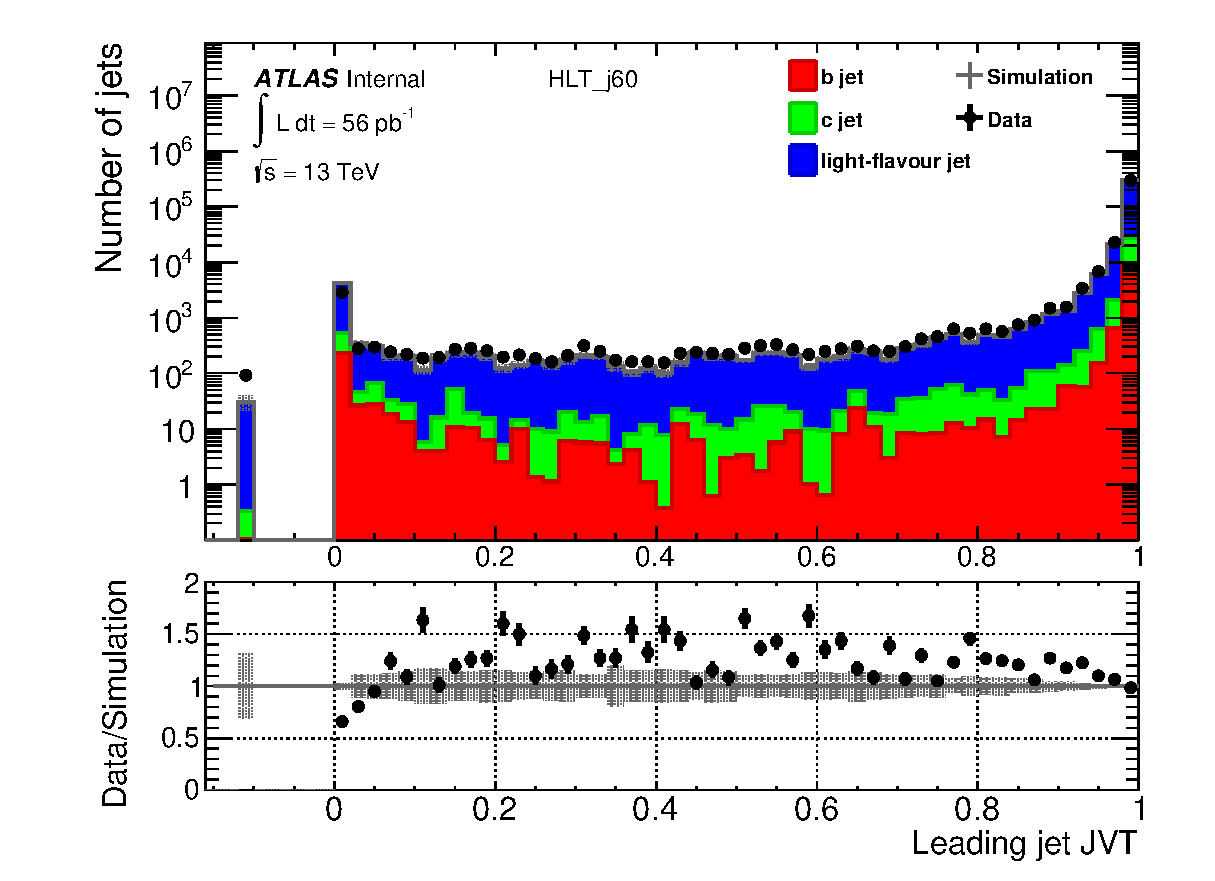
\includegraphics[width=0.45\textwidth]{plots/LeadingJet/JVT.eps}
	 \caption{Distributions of $p_{T}$ (left) and $\eta$ (right)
           %, number of associated tracks (bottom left) and JVT (bottom right) 
           for the leading jet, for data (solid points) and simulation (grey shaded) 
           which is shown as a stack of its flavour components; \textit{b}, \textit{c} and light flavoured jets (red, green and blue respectively).}
         \label{LeadJetKine}
  \vspace{-0.2cm}
\end{figure}


\subsection{Tracking}

As discussed in Section \ref{s_ATLAS} and \ref{s_Algos} tracks from the inner detector are crucial to all flavour tagging algorithms.
Between Run-1 and Run-2 there have been changes to the tracking, most notably the introduction of the IBL.
Hence, the tracking performance of the Run-2 data must be studied.
%Figure \ref{TrackHits} shows the average number of hits in the IBL for a track as functions of $\phi$, $\eta$ and track-$p_{T}$ for data and simulation.
In general the tracking distributions show good agreement between data and simulation; however some improvements in the understanding are required.
A further discussion of issues relating to tracking per
formance is in Section \ref{sss_comm_perf_IPxD}.

%\begin{figure}[!htb]
%	 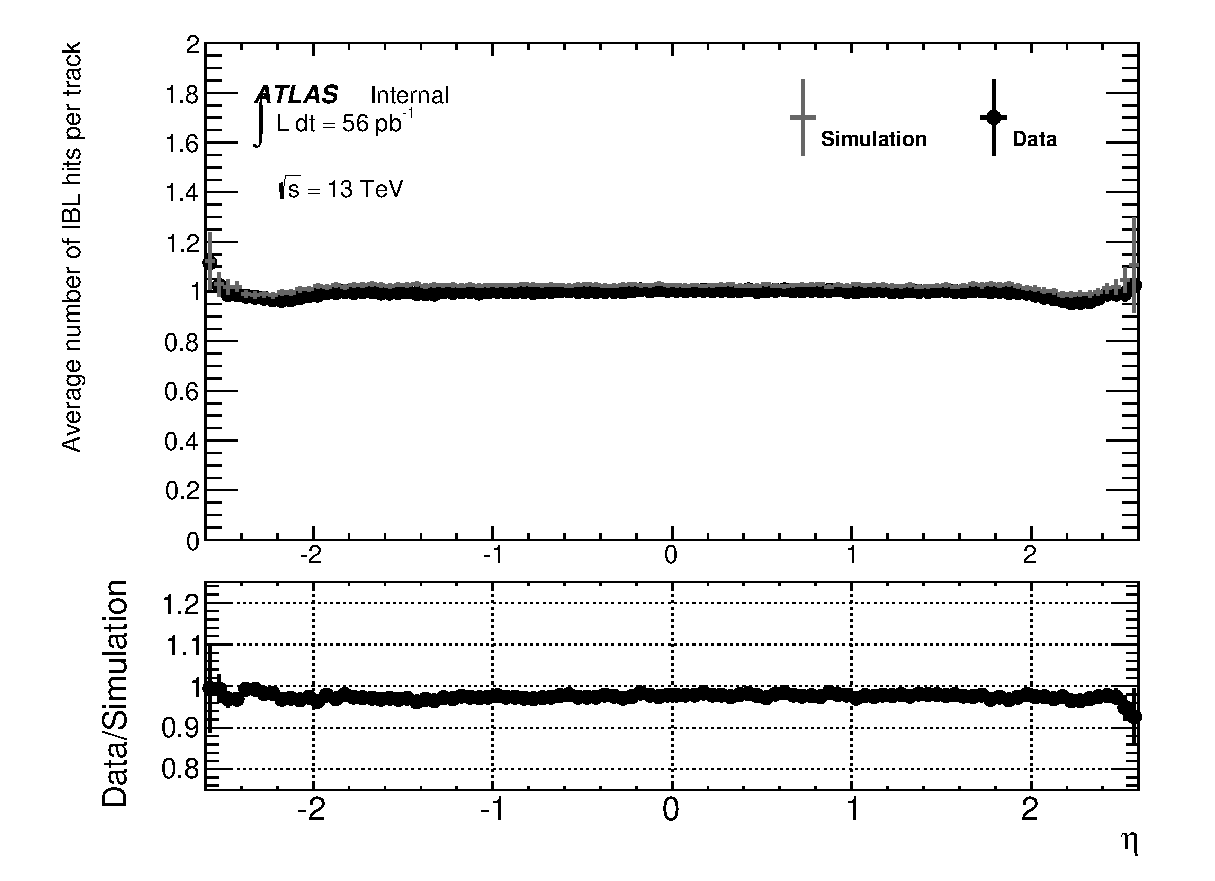
\includegraphics[width=0.45\textwidth]{plots/TrackHit/trk_nInnHits_eta.eps}
%	 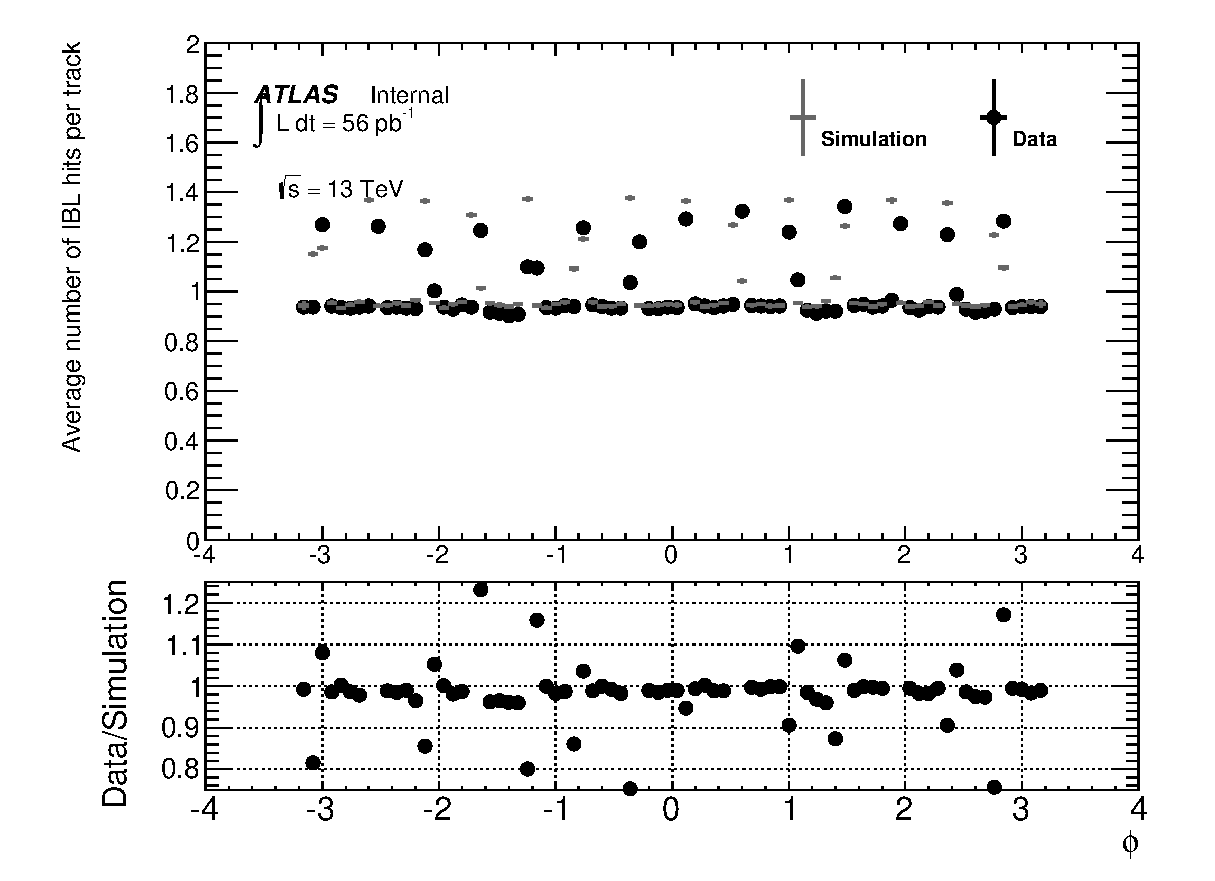
\includegraphics[width=0.45\textwidth]{plots/TrackHit/trk_nInnHits_phi.eps}
         %\\\center 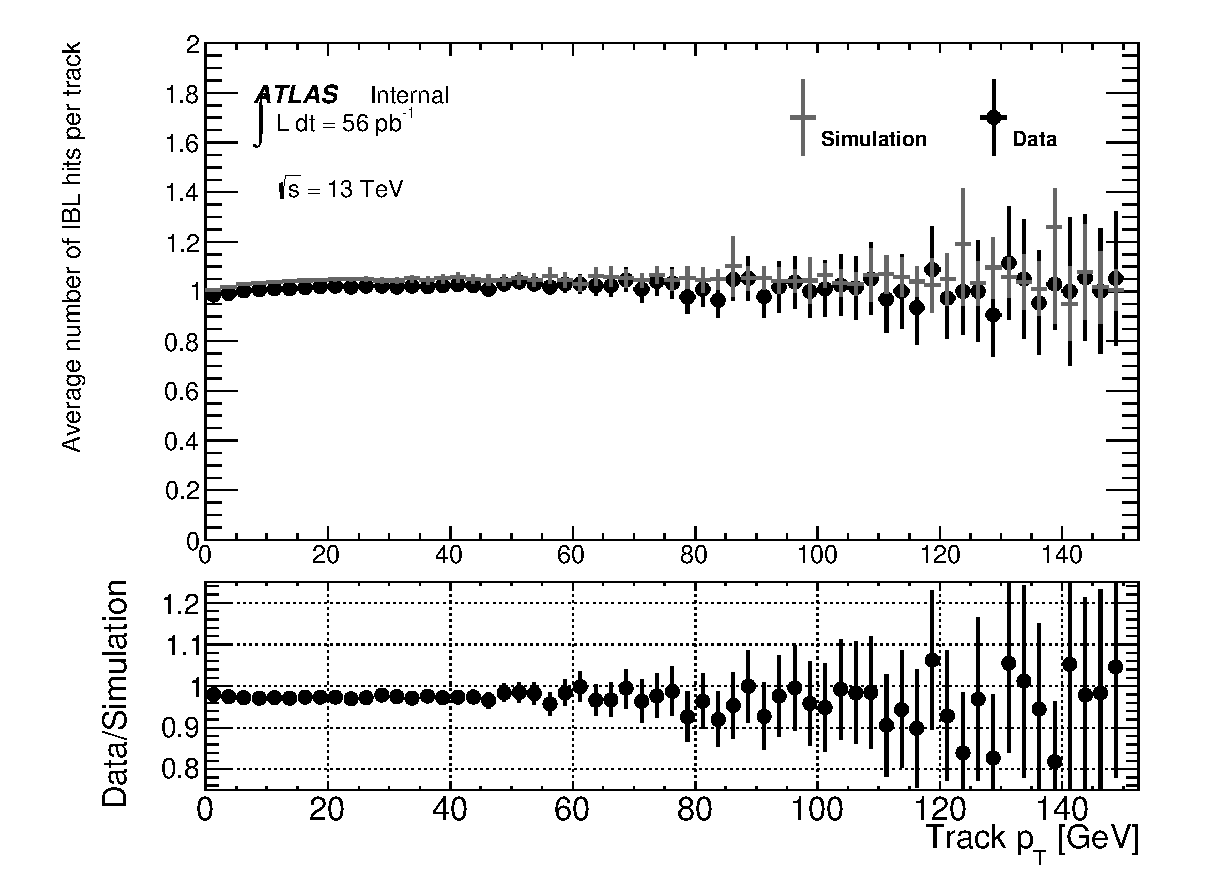
\includegraphics[width=0.45\textwidth]{plots/TrackHit/trk_nInnHits_pt.eps}
%	 \caption{Distributions of the average number of IBL hits per track against $\eta$ (top left) and $\phi$ (top right) 
           %and $p_{T}$ (bottom) for the leading jet;
%           for data (solid points) and simulation (grey shaded).}
%         \label{TrackHits}
%         \vspace{-0.5cm}
%\end{figure}

\subsection{Flavour Tagging Algorithm Performance} \label{ss_comm_perf}

Below I will study the key properties of the each of the three base flavour algorithms as well as the multivariate algorithm MV2, as described in Section \ref{s_Algos}.

\subsubsection{IPxD} \label{sss_comm_perf_IPxD}

Figure \ref{IP} shows the distributions of $d_0$, $z_0$, $d_0$ significance and $z_0$ significance, which are the key features of the IP2D and IP3D algorithms,
as discussed in Section \ref{ss_Algos_IPxD}.
Here there are significant discrepancies between data and simulation. 
The discrepancies in the $d_0$ and $z_0$ distributions are likely due to misalignments of the inner detector; 
where a mismodelling of the position of the detector components relative to each other and to the beam-line in the tracking software 
means that tracks are not accurately reconstructed in data.
The discrepancies in the $d_0$ and $z_0$ significance distributions are likely due to a combination of the misalignment discussed above
and the fact that there is IBL material missing in the ATLAS model used in the simulation, meaning that impact parameter errors are miscalculated.

\begin{figure}[!htb]
	 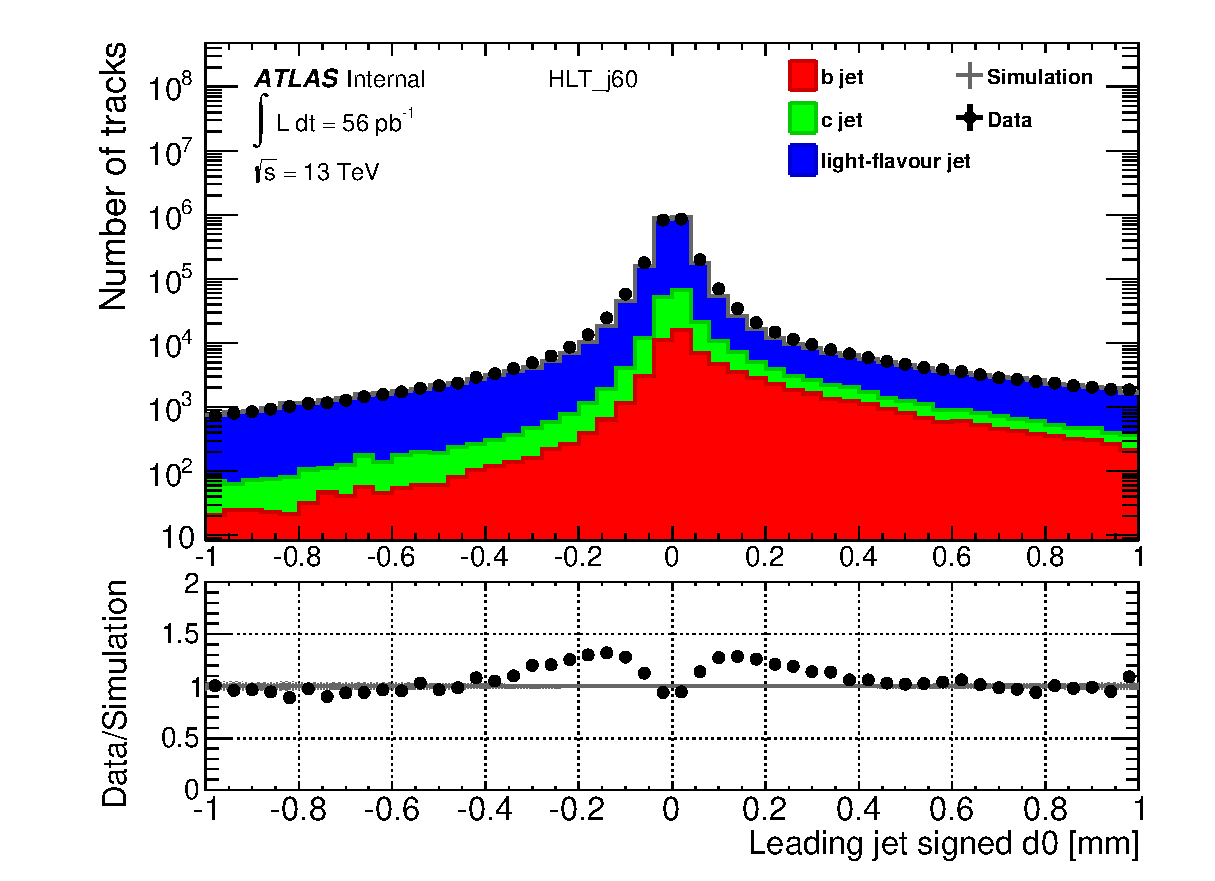
\includegraphics[width=0.45\textwidth]{plots/LeadingJet/trk_ip3d_d0.eps}
	 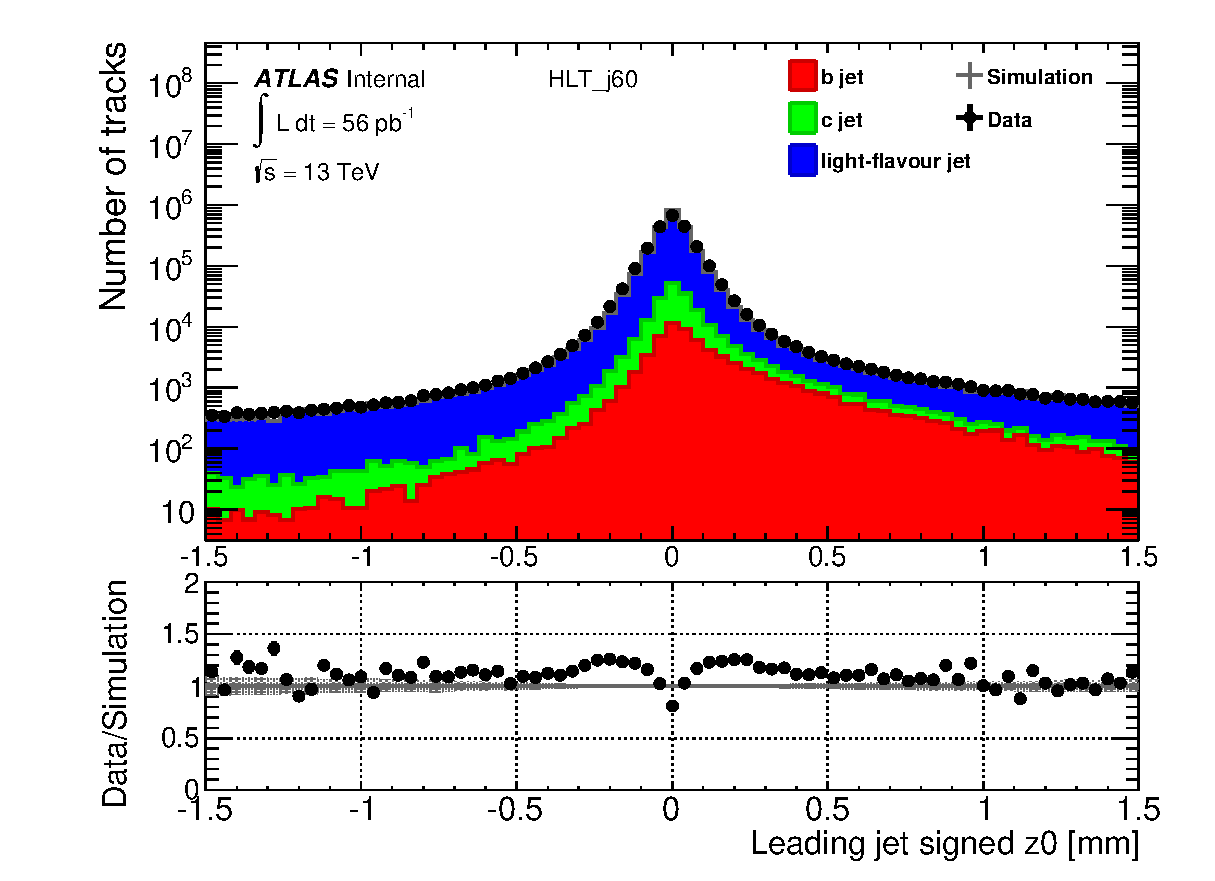
\includegraphics[width=0.45\textwidth]{plots/LeadingJet/trk_ip3d_z0.eps}\\
         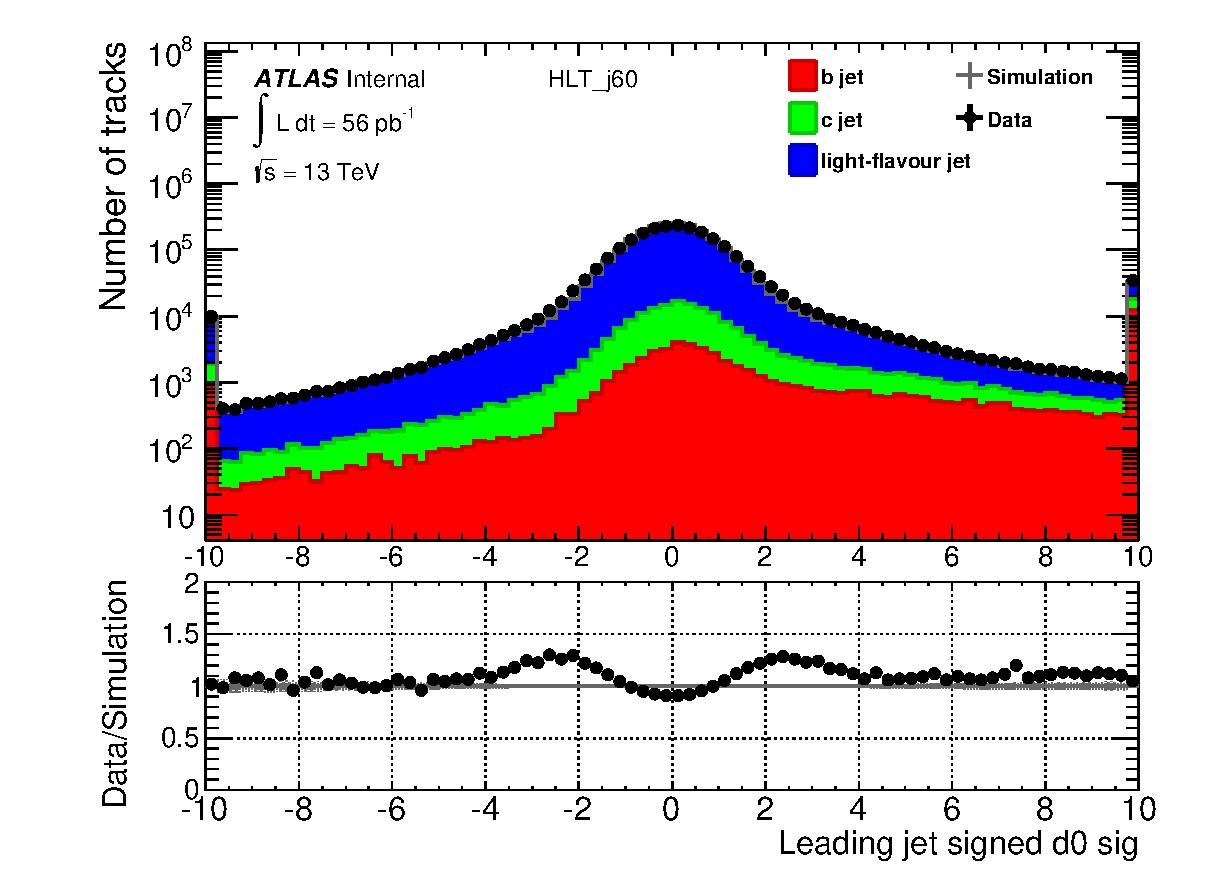
\includegraphics[width=0.45\textwidth]{plots/LeadingJet/trk_ip3d_d0sig.eps}
         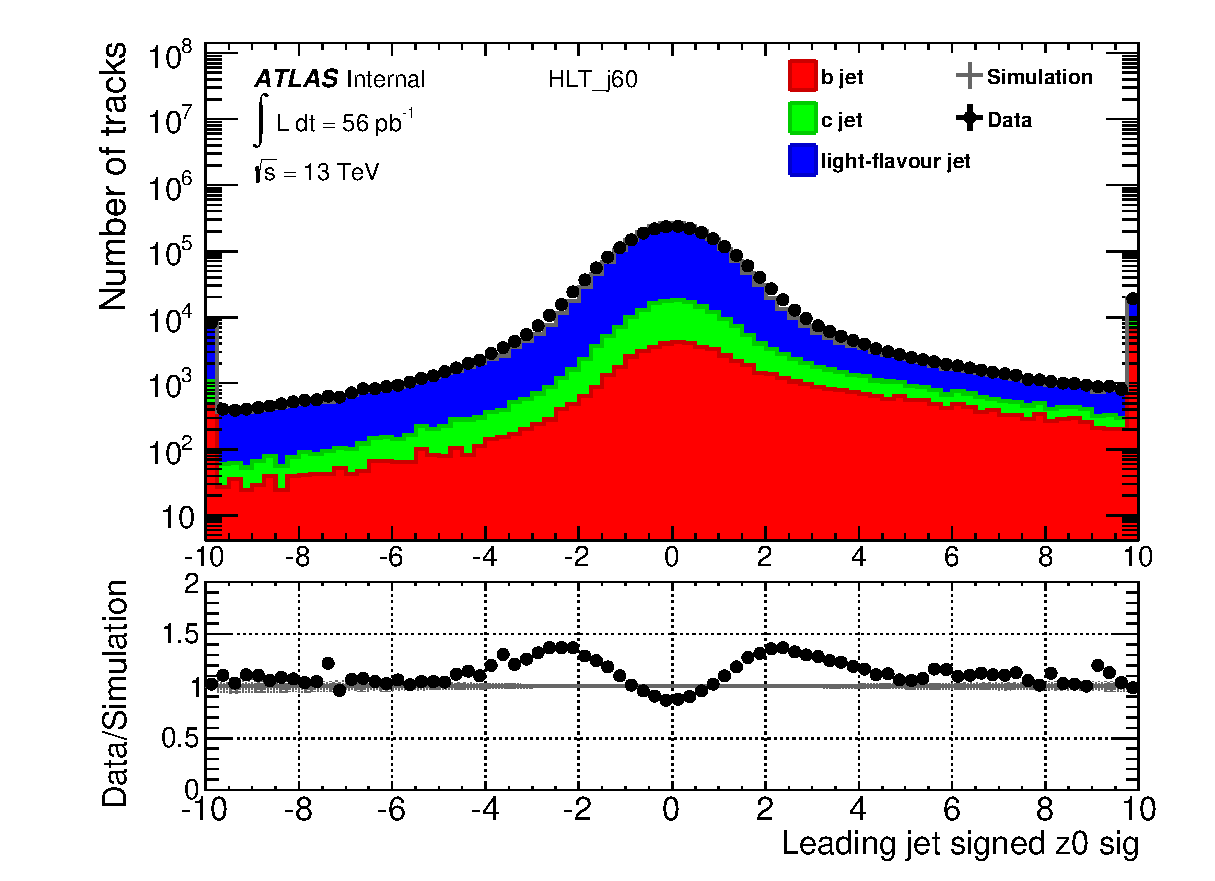
\includegraphics[width=0.45\textwidth]{plots/LeadingJet/trk_ip3d_z0sig.eps}
	 \caption{Distributions of $d_0$ (top left), $z_0$ (top right), $d_0$ significance (bottom left) and $z_0$ significance (bottom right) 
           for the leading jet, for data (solid points) and simulation (grey shaded) 
           which is shown as a stack of its flavour components; \textit{b}, \textit{c} and light flavoured jets (red, green and blue respectively).}
         \label{IP}
  %\vspace{-1cm}
\end{figure}

\subsubsection{SV1}

As discussed in Section \ref{ss_Algos_SV1}, the inputs to MV2 from SV1 are the properties of the constructed vertex that demonstrate flavour discrimination.
Figure \ref{SV1} shows the key variables of SV1 for the leading jet, if a secondary vertex is found; the vertex invariant mass (SV mass), vertex energy fraction, the 2D flight path ($L_{XY}$) 
and the number of tracks at the vertex. In general SV quantities show good agreement between simulation and data.

\begin{figure}[!htb]
         \vspace{-0.2cm}
	 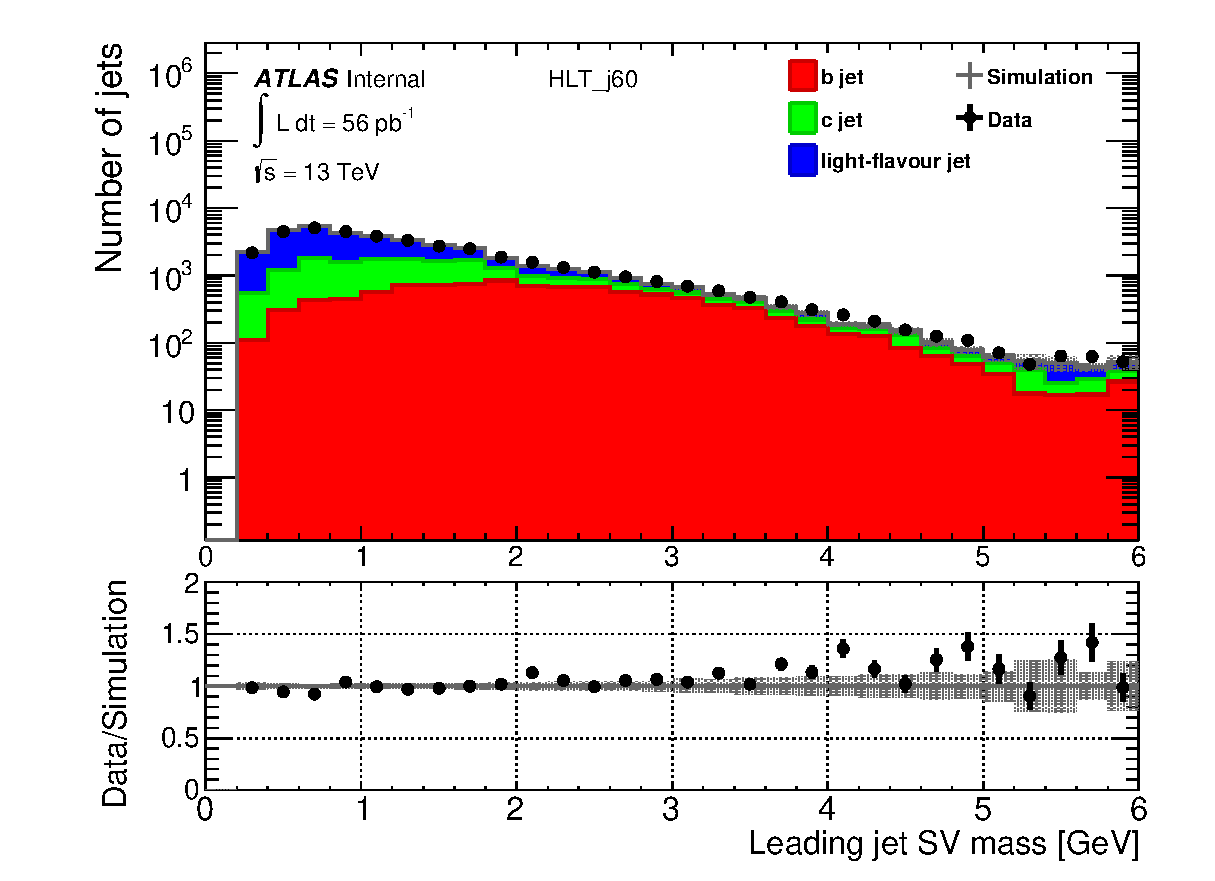
\includegraphics[width=0.45\textwidth]{plots/LeadingJet/sv1_m.eps}
	 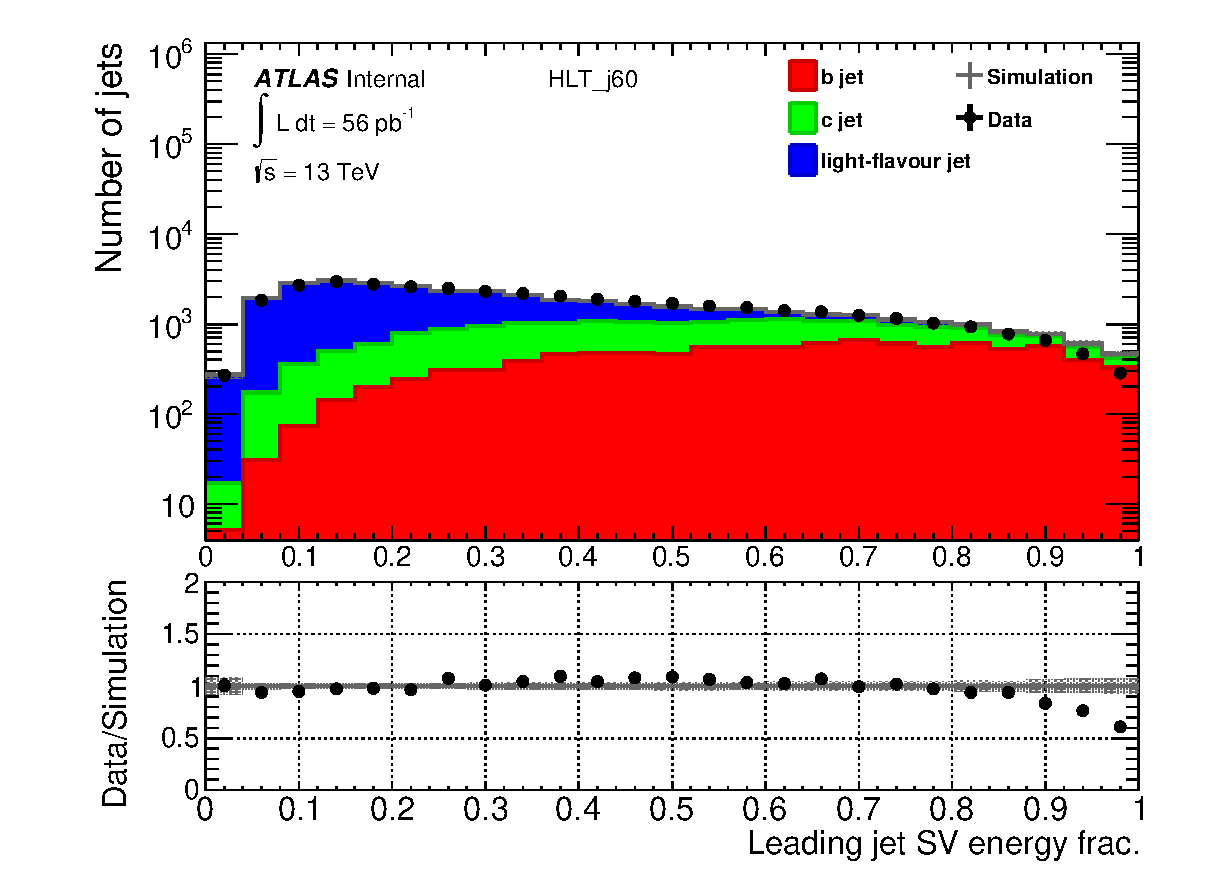
\includegraphics[width=0.45\textwidth]{plots/LeadingJet/sv1_efc.eps}\\
         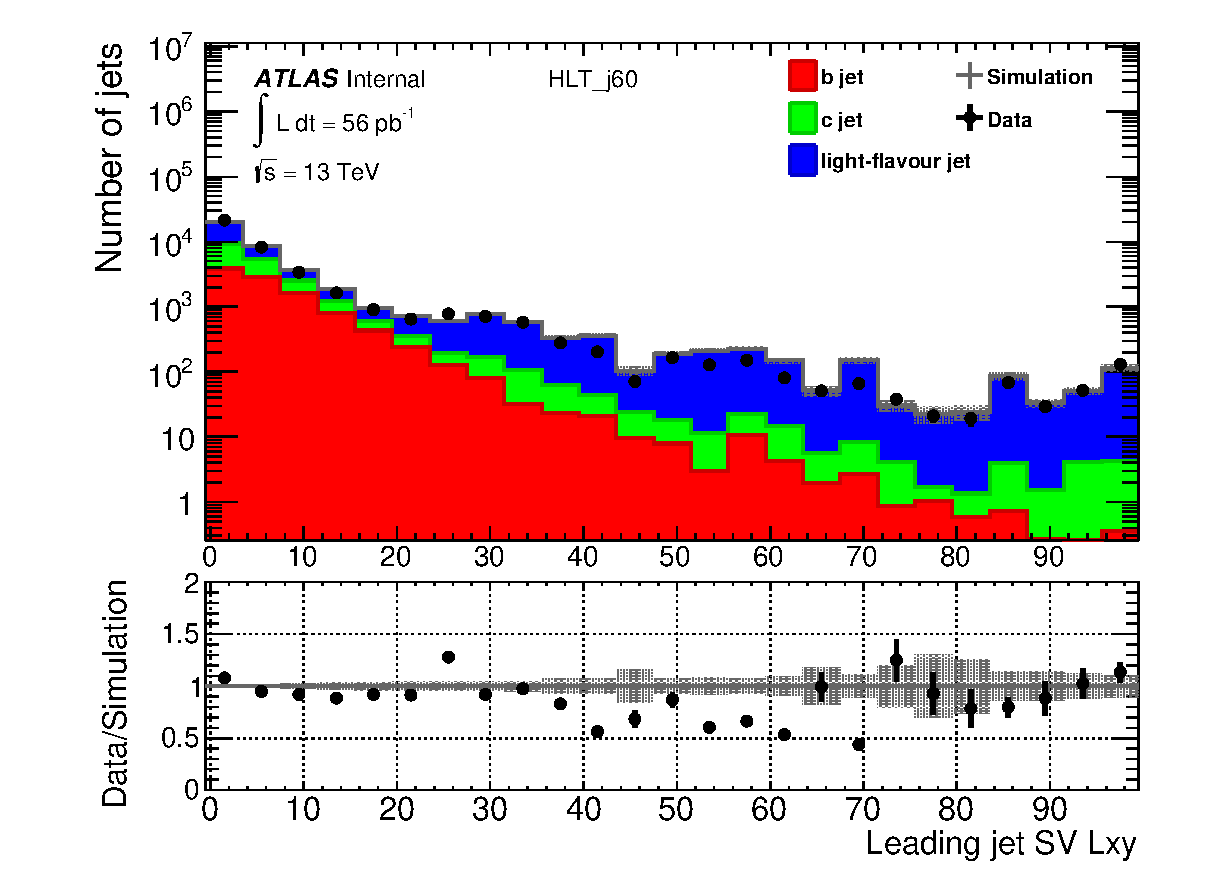
\includegraphics[width=0.45\textwidth]{plots/LeadingJet/sv1_Lxy.eps}
         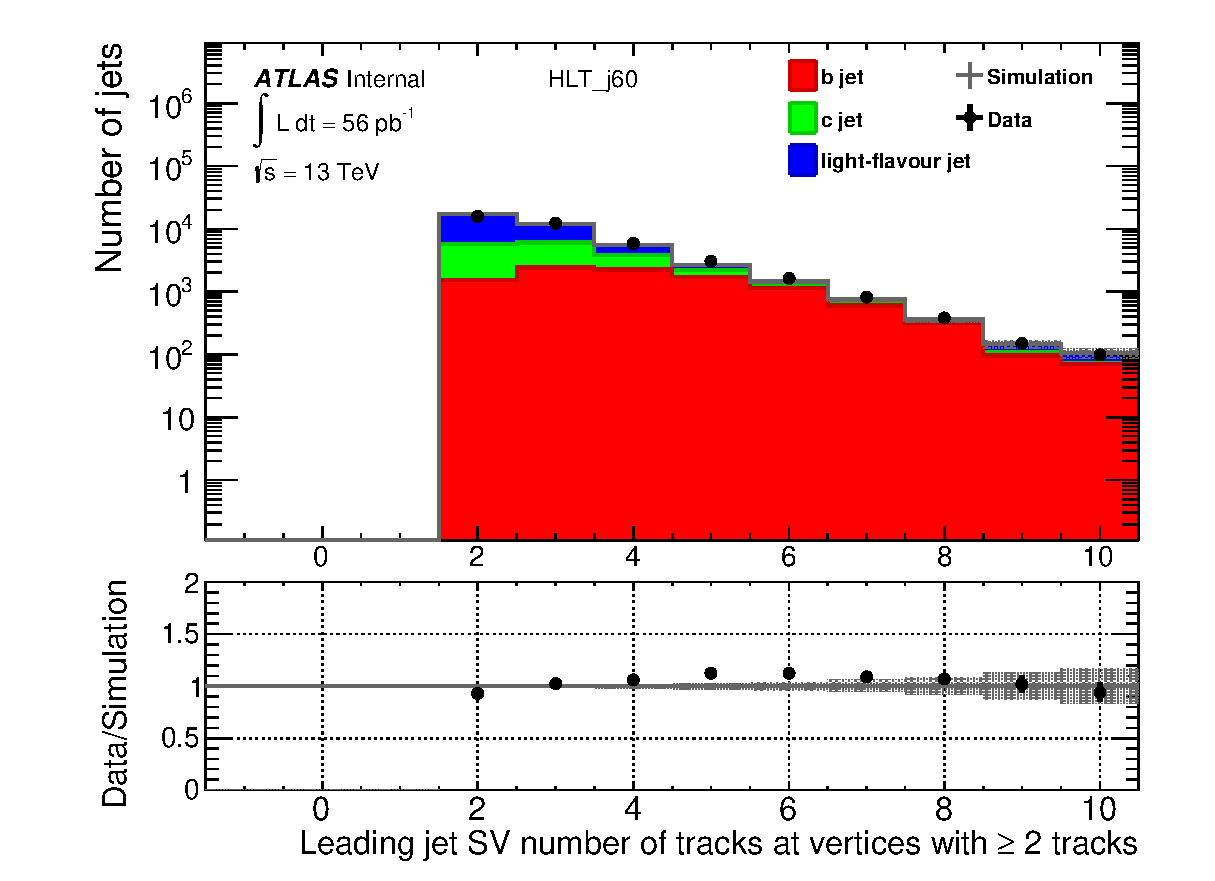
\includegraphics[width=0.45\textwidth]{plots/LeadingJet/sv1_ntrkv.eps}
	 \caption{Distributions of SV vertex mass (top left), energy fraction (top right), 2D flight path (bottom left) and number of tracks at vertices (bottom right)
           for data (solid points) and simulation (grey shaded) 
           which is shown as a stack of its flavour components; \textit{b}, \textit{c} and light flavoured jets (red, green and blue respectively).}
         \label{SV1}
         \vspace{-0.6cm}
\end{figure}

\subsubsection{JetFitter}

As discussed in Section \ref{ss_Algos_JF}, the inputs to MV2 from JF are the properties of the constructed vertices that demonstrate flavour discrimination.
Figure \ref{JF} shows the key variables of JF for the leading jet, if at least one vertex found;
the invariant mass of the vertices (JF mass), energy fraction of the vertices, the number of vertices with two or more tracks
and the number of one track vertices. JF variables show reasonable agreement between simulation and data.

\begin{figure}[!htb]
	 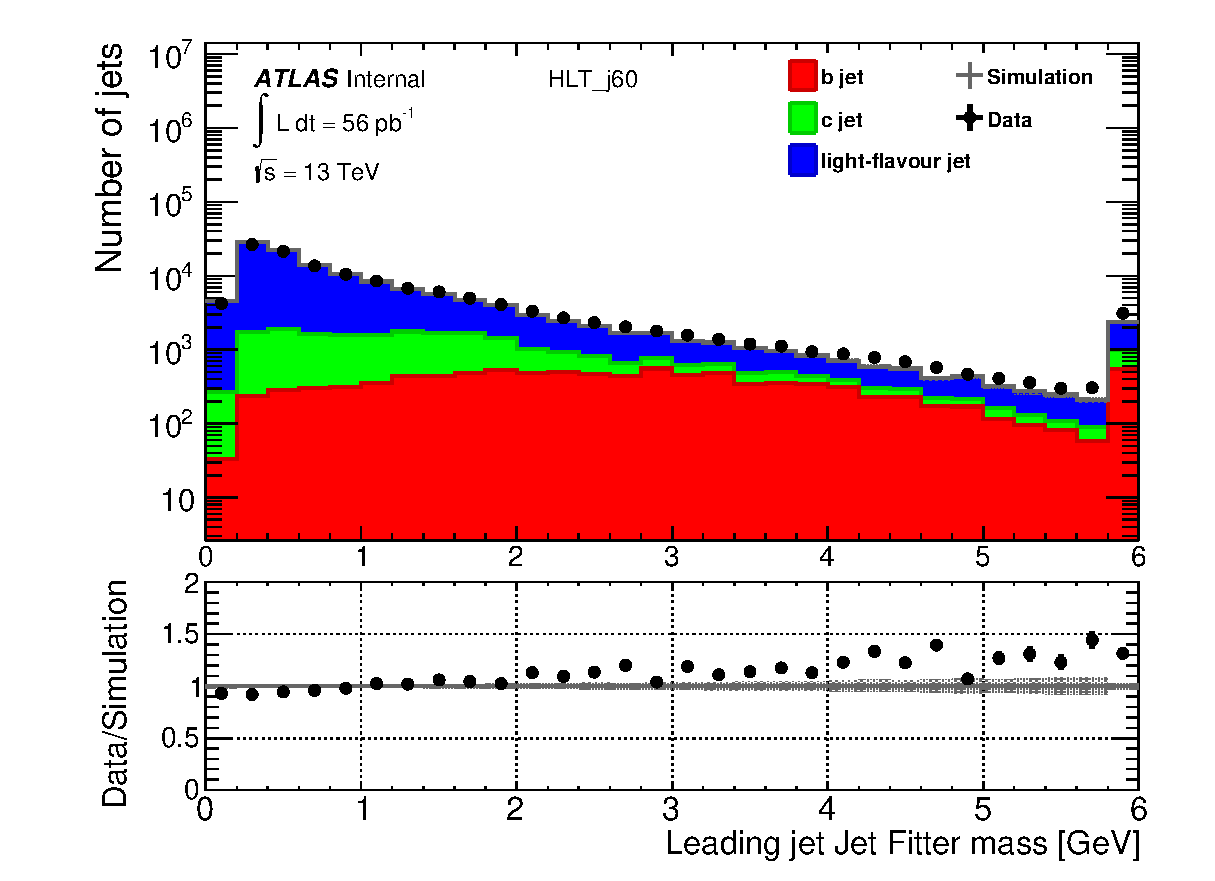
\includegraphics[width=0.45\textwidth]{plots/LeadingJet/jf_m.eps}
	 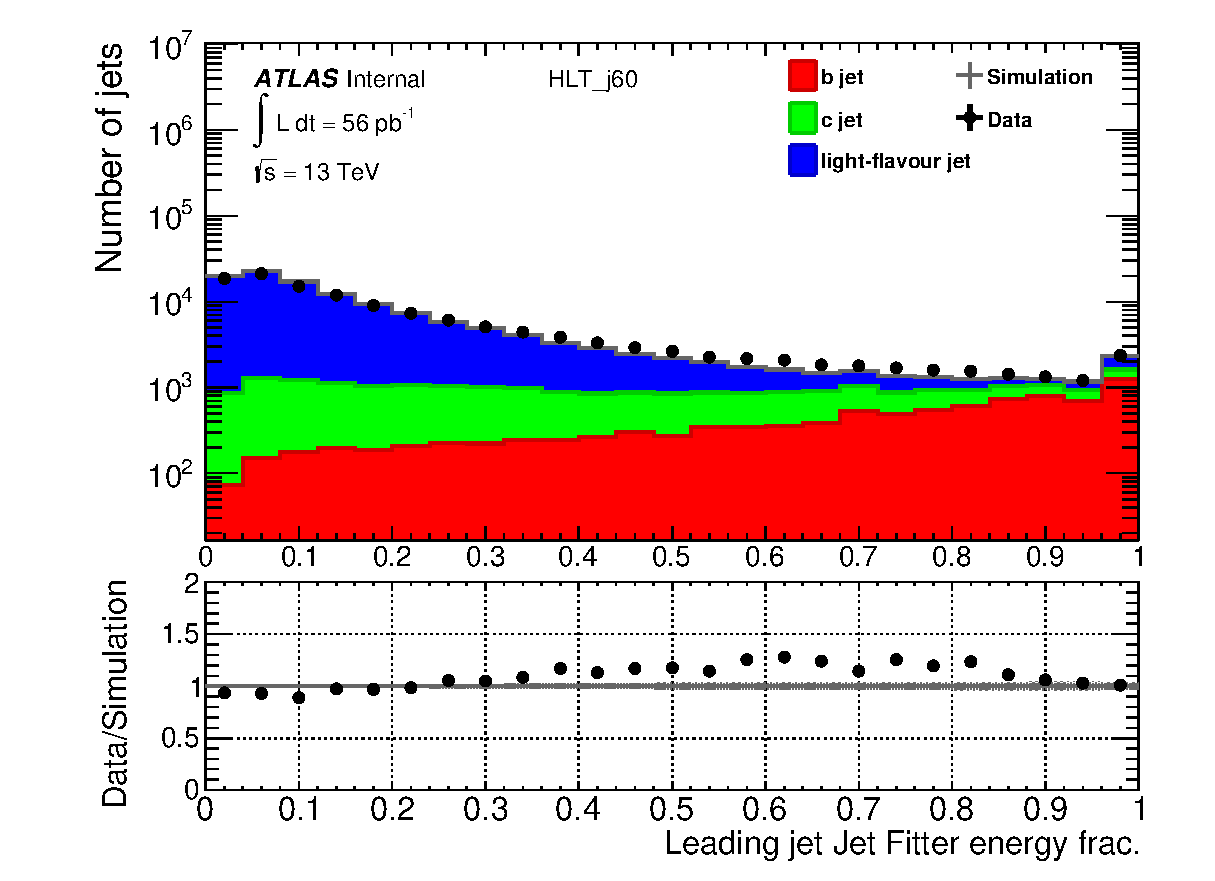
\includegraphics[width=0.45\textwidth]{plots/LeadingJet/jf_efc.eps}\\
         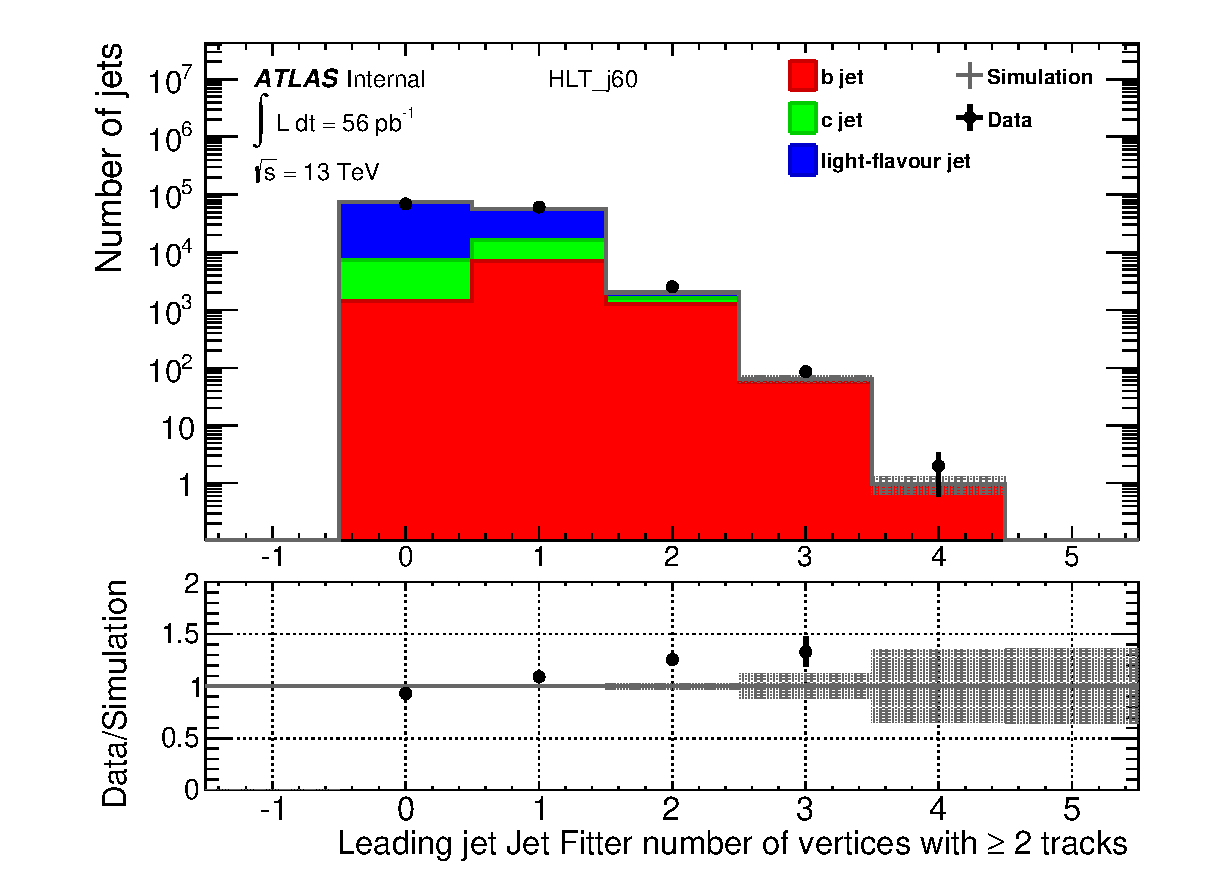
\includegraphics[width=0.45\textwidth]{plots/LeadingJet/jf_nvtx.eps}
         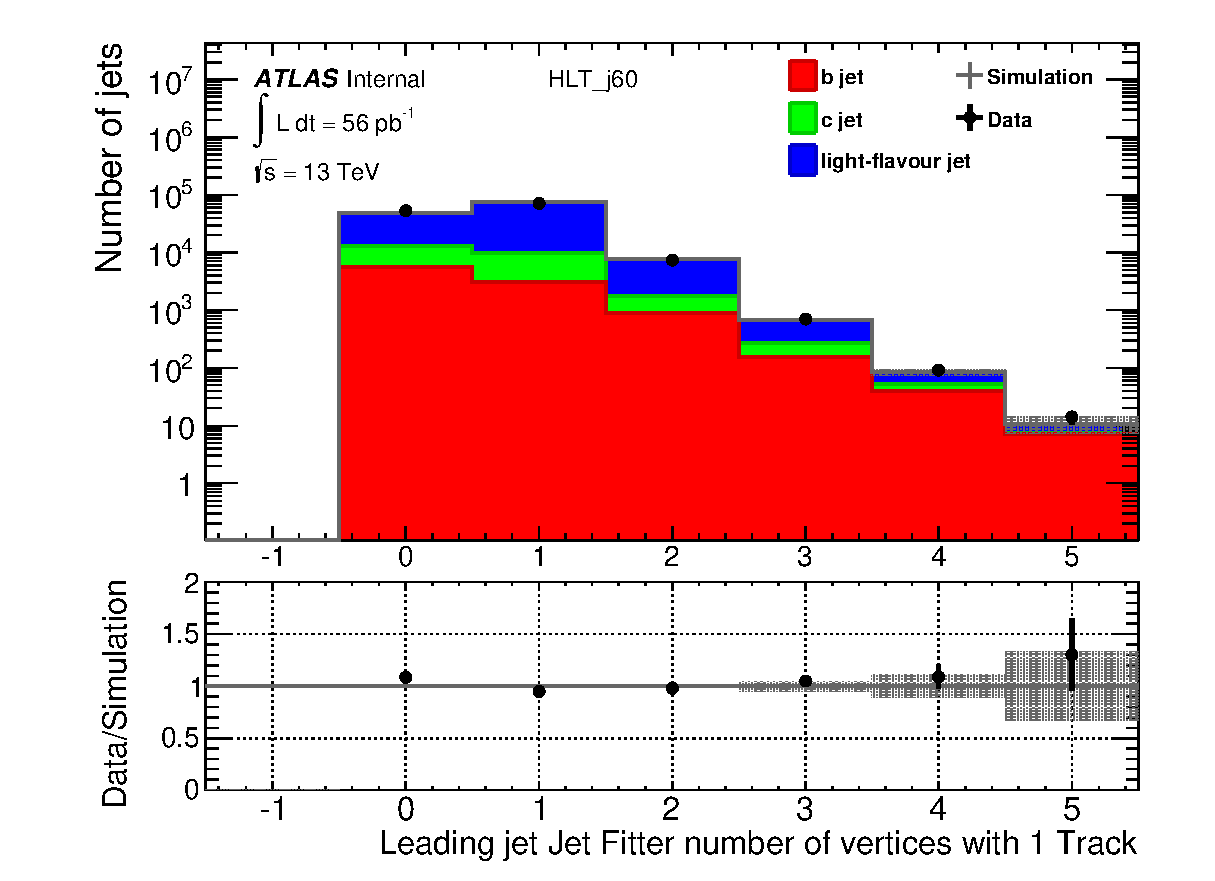
\includegraphics[width=0.45\textwidth]{plots/LeadingJet/jf_nvtx1t.eps}
	 \caption{Distributions of JF vertex mass (top left), energy fraction (top right), number of vertices with at least two tracks (bottom left)
           and the number of one track vertices (bottom right) for the leading jet, for data (solid points) and simulation (grey shaded) 
           which is shown as a stack of its flavour components; \textit{b}, \textit{c} and light flavoured jets (red, green and blue respectively).}
         \label{JF}
  %\vspace{-1cm}
\end{figure}

\subsubsection{MV2c20}

The recommended tagger for Run-2 is MV2c20, as discussed in Section \ref{ss_Algos_MV2}.
The left plot in Figure \ref{MV2} shows MV2c20 for the leading jet; there is a discrepancy in the lowest bin, 
which then causes the overall normalisation to be incorrect in the rest of the bins. 

\begin{table}[!htb]
  \vspace{+0.2cm}
  \begin{center}
    \begin{tabular}{ | c | c || c | c | c | }
      \hline
      Working Point & Jet Type  & Fraction of \textit{b}-jets &  Fraction of \textit{c}-jets & Fraction of light\\
      \hline

      100\% & Leading    & 0.03056 $\pm$ 0.00072 & 0.05909 $\pm$ 0.00052 & 0.91034 $\pm$ 0.00013 \\
            & Subleading & 0.03346 $\pm$ 0.00070 & 0.06256 $\pm$ 0.00052 & 0.90398 $\pm$ 0.00014 \\
      \hline
      70\%  & Leading    & 0.65079 $\pm$ 0.00084 & 0.27604 $\pm$ 0.00129 & 0.07317 $\pm$ 0.00250 \\
            & Subleading & 0.13689 $\pm$ 0.00189 & 0.06873 $\pm$ 0.00267 & 0.79437 $\pm$ 0.00079 \\
      \hline
    \end{tabular}
    \caption{The fractions of jet flavours for the leading and subleading jet when no tag is applied (working point of 100\%) and
      for the b-enhance sample, when a tag of MV2c20 at $\epsilon_{b}$ = 70\% is applied to the leading jet (working point of 70\%). }
    \label{benhance_table}
    \vspace{-0.8cm}

  \end{center}
\end{table}


In addition a sample that is enhanced in \textit{b}-jets is also studied, as this allows a closer examination of the 
modelling of the flavour tagging algorithms as applied to \textit{b}-jets.
To create an unbiased sample that is enhanced in \textit{b}-jets, MV2c20 is used to tag the leading jet with \textit{b}-efficiency of 70\%, which corresponds
to light- and \textit{c}-jet rejection rates of $\sim$440 and $\sim$8, respectively. 
However, the leading jet is now biased, as we have selected jets that have properties that give a high MV2c20 value.
Instead, by using the subleading jet partner of the tagged leading jet, due to flavour correlation in QCD, we have a sample of jets that have an enhanced \textit{b}-jet fraction,
but are not biased by the use of an algorithm tag.
Table \ref{benhance_table} shows the flavour fractions of leading and subleading jet before and after the tag is applied.
The MV2c20 distribution of the b-enhanced sample is shown on the right in Figure \ref{MV2}. The agreement between data and simulation 
for MV2c20 in the b-enhanced sample is improved compared to the full sample shown on the left. 
The reason for this improvement is not well understood and is under further investigation.



\begin{figure}[!htb]
	 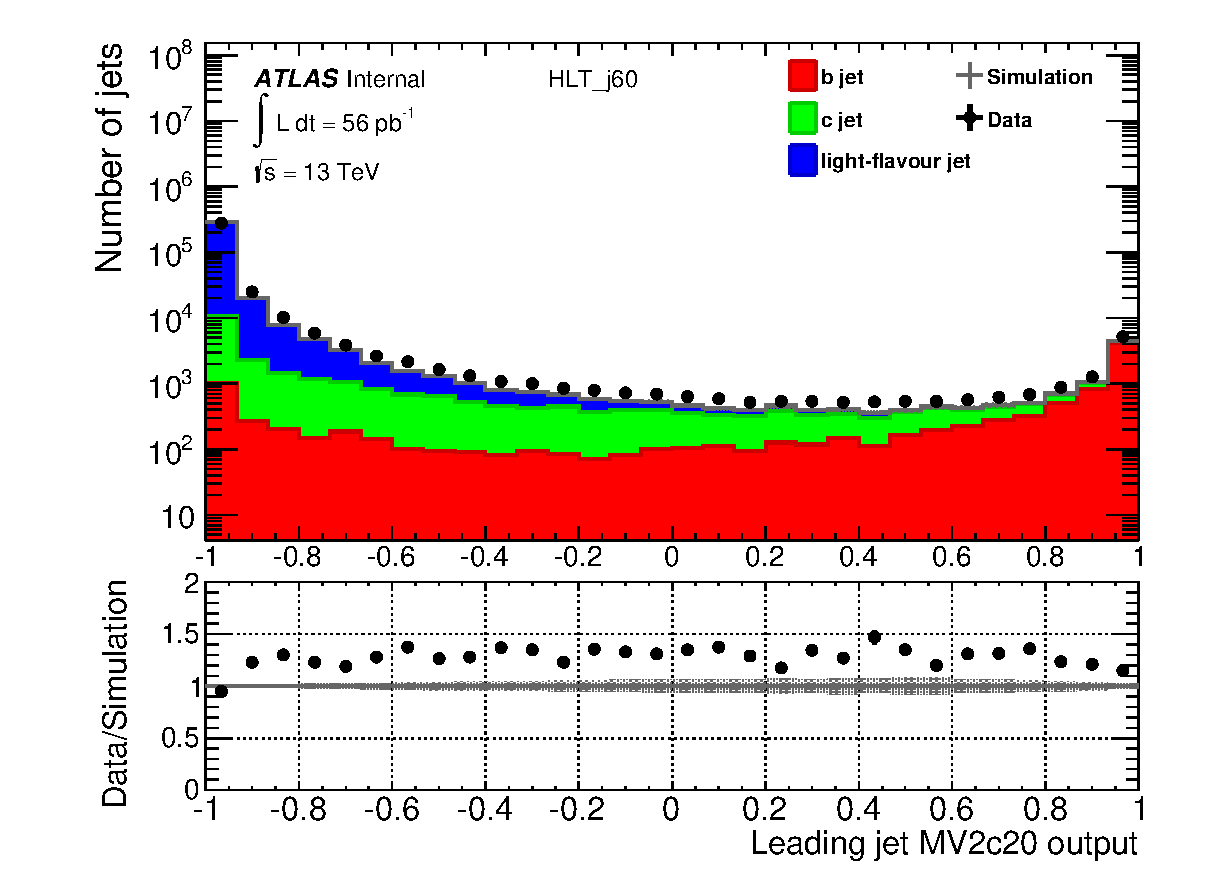
\includegraphics[width=0.45\textwidth]{plots/LeadingJet/mv2c20.eps}
	 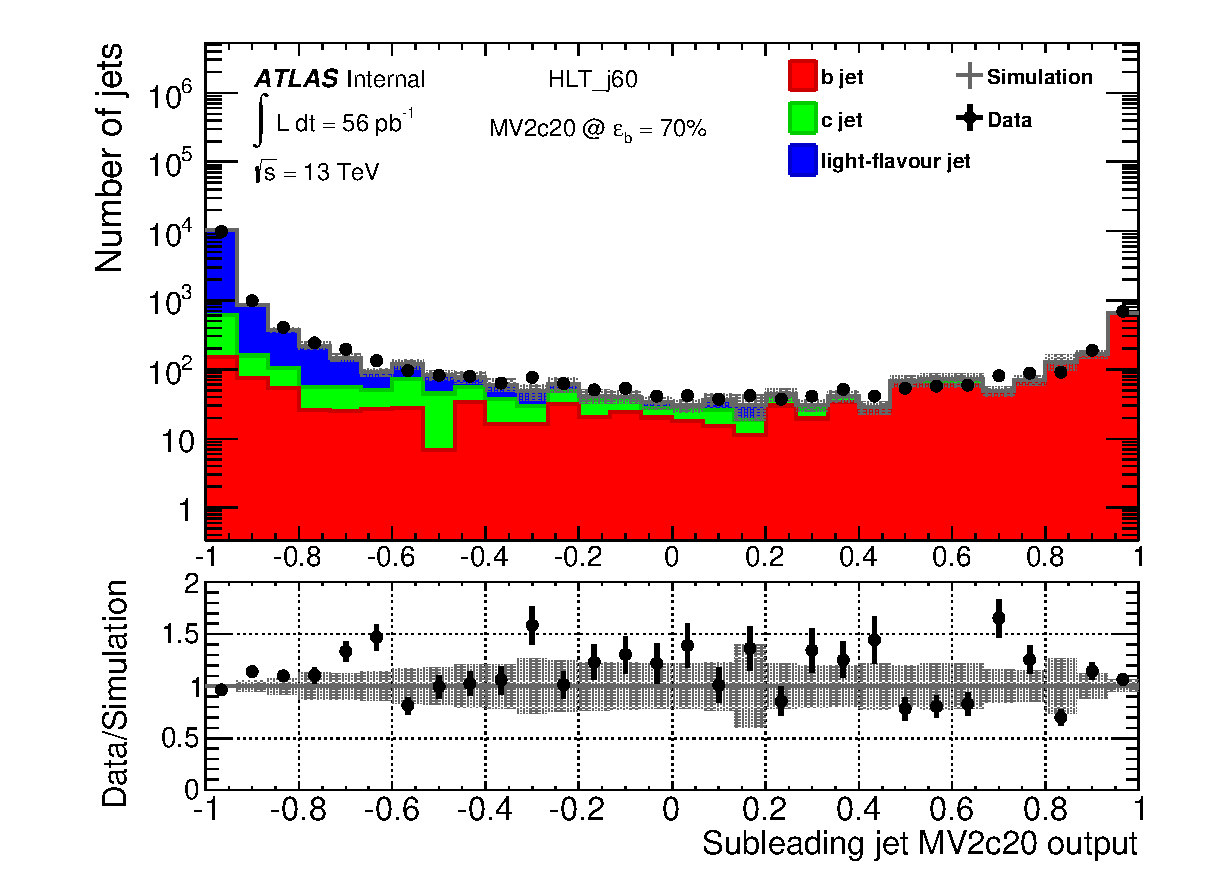
\includegraphics[width=0.45\textwidth]{plots/bEnhance_70_SubLeadingJet/mv2c20_sublead.eps}
	 \caption{Distributions of MV2c20 output for the leading jet when no tag is applied (left), 
           and for the subleading jet when a 70\% efficiency MV2c20 tag is applied to the leading jet (right),
           for data (solid points) and simulation (grey shaded) 
           which is shown as a stack of its flavour components; \textit{b}, \textit{c} and light flavoured jets (red, green and blue respectively).}
         \label{MV2}
\end{figure}



\section{High jet-$p_{T}$ \textit{b}-Tagging Performance} \label{s_high_pt_btag}

Many searches for beyond standard model physics at ATLAS focus on searches for large mass particles 
($m \sim 1$ TeV), as this uses previously unexplored regions of phase-space.
Objects from the decay of these particles will be at higher $p_T$ and, as discussed in the Introduction,
\textit{b}-tagging features in many of these analyses.
Hence, in many of these searches \textit{b}-tagging of high-$p_{T}$ jets is important, such as the di-b-jet resonant search discussed in Section \ref{s_dibjet}.
However, \textit{b}-tagging performance drops significantly at high-$p_{T}$, which means that for the same \textit{b}-jet efficiency, 
there is a fall in light-rejection rate \footnote{Light-rejection rate is the number of truth light-flavoured jets per truth 
light-flavoured jet falsely tagged as \textit{b}-jet.}.
This is due to a number of factors: tracks have larger uncertainties on track parameters at high-$p_T$ and 
there are difficulties in reconstructing vertices as tracks have higher collimation in boosted high-$p_T$ jets.
%This drop in \textit{b}-tagging performance can be seen in Figure \ref{b-tag_high_pt}, 
%which shows that for a fixed efficiency cut of $\epsilon_b$ = 70\% for MV2c20, the light-rejection rate
Improving \textit{b}-tagging performance at high-$p_T$ would in turn improve the sensitivity of the searches that depend on high-$p_T$ b-tagging. \\

%\begin{figure}[!htb]
%  \begin{center}
%	 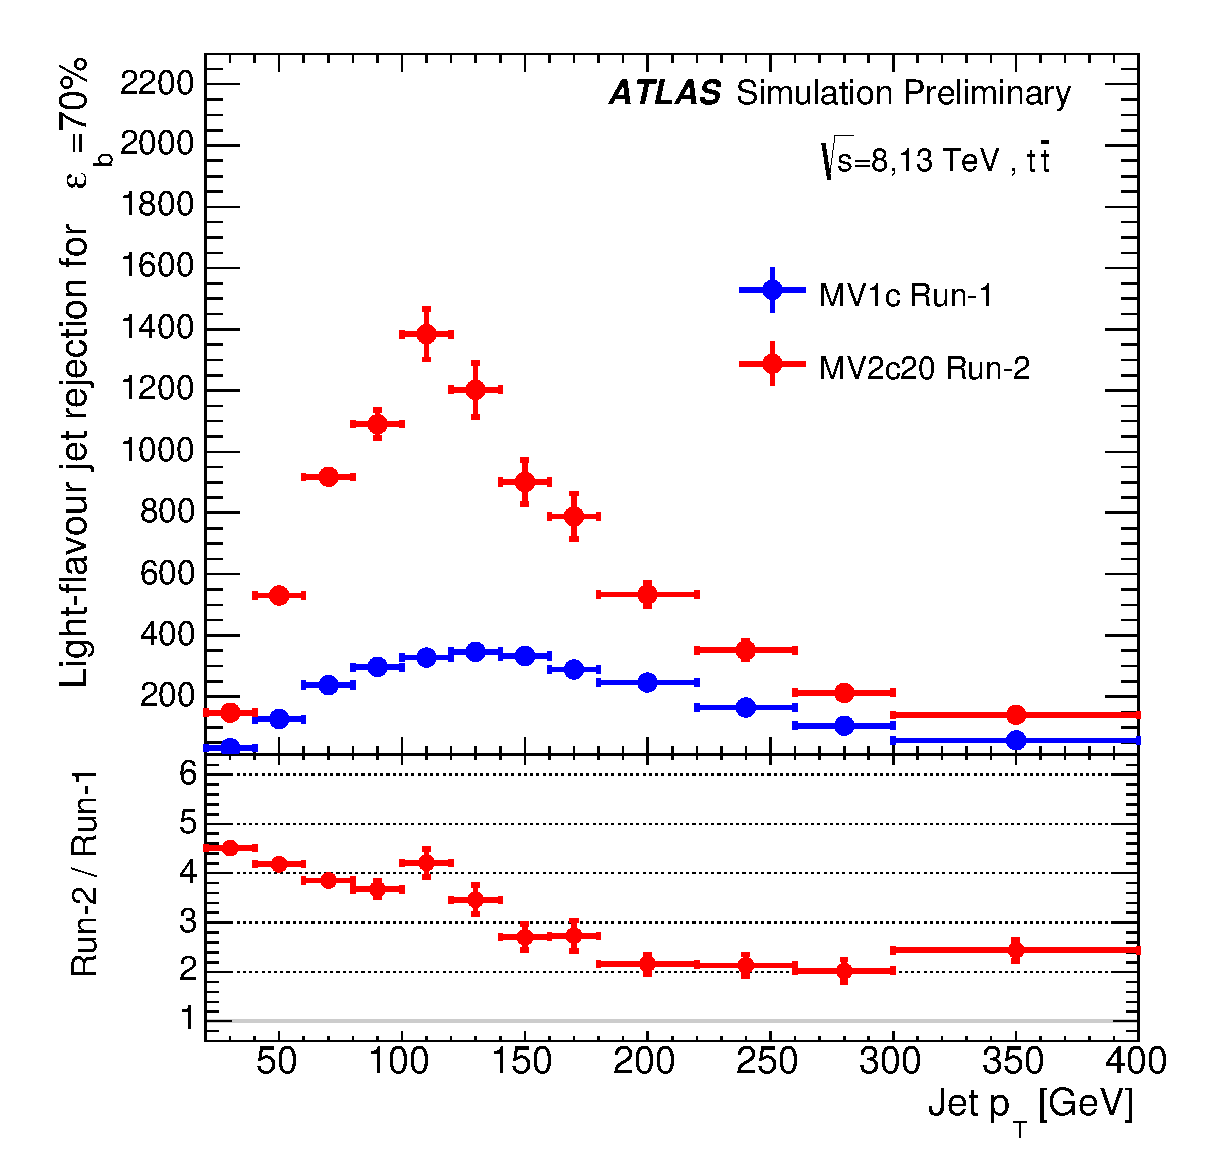
\includegraphics[width=0.4\textwidth]{figures/b-tag_high_pt.eps}
%	 \caption{The light-rejection rate as a function of $p_T$ for the MV1c b-tagging algorithm used in Run-1 (blue) compared to the MV2c20 b-tagging algorithm using the Run-2 setup (red). 
%           In each pT  bin the b-tagging cut value has been chosen in such a way to yield a constant b-jet efficiency of 70\%}
%         \label{b-tag_high_pt}
%  \end{center}
%\end{figure}

One possible improvement is to consider the set of track cuts used by the base algorithms.
For a track to be considered by an algorithm it must pass a series of cuts, that are designed to 
reduce the number of fake or pile-up tracks and ensure the quality of tracks considered by the algorithm.
For IP3D, the set of cuts applied to tracks is shown in Table \ref{track_cuts}, 
which will be referred to as the IP3D track cuts for the remainder of this report.
By re-tuning the track selection for high $p_T$ jets, improvements in \textit{b}-tagging performance at high jet-$p_T$ may be possible. \\

\begin{table}[!htb]
  
  \vspace{-0.2cm}
  \begin{center}
    \begin{tabular}{ | c | c | c | c | c | c | c  }
      \hline
      Track-$p_T$ & $|\eta|$  & \# SCT Hits + \# Pixel Hits &  \# Pixel Hits & $d_0$ & $z_0 Sin(\theta)$\\
      \hline
      $>$ 1 GeV  & $<$ 2.5  & $\geq 7$ & $\geq 2$ & $< 1$ & $< 1.5$\\
      %\hline
     
      \hline
    \end{tabular}
    \caption{The set of track cuts used by the IP3D algorithm to select tracks.}
    \label{track_cuts}
    \vspace{-0.6cm}

  \end{center}
\end{table}

In this study, a simulated sample of the decay of a Z'-boson to $b\bar{b}$ is used,
where the Z'-boson is a theoretical boson proposed by various models, discussed further in Section \ref{s_dibjet}.
As the mass of the Z'-boson is a free parameter, we use a 
sample containing Z'-bosons with a mass of 
1, 2, 3, 4 and 5 TeV, such that the decay of these particles gives a sample containing \textit{b}-jets up to very high jet $p_T$. 
The sample is simulated using the same set up as described in Section \ref{ss_comm_simulation}.
Jets are reconstructed and calibrated using the same set-up described in Section \ref{ss_comm_event},
except that a jet must have $p_{T} > $ 25 GeV, $|\eta| <$ 2.5 and no JVT output cut is applied. \\

Tracks in \textit{b}-jets can have several origins;
the decay of the \textit{b}-hadron (including the decay of the subsequent \textit{c}-hadron),
the initial parton shower and hadronisation process of the jet, pile-up and fakes, and from interactions of particles with the material in the detector.
The tracks from the different origins are labelled as from B, from Fragmentation, from Pile-up/Fake (PuFake) and from Geant respectively.
As tracks from B are the tracks from the \textit{b}-hadron, these are the tracks with the properties that show discrimination between jet flavours, 
such as offset vertices and large impact parameters. 
Hence a set of cuts that maximise the fraction of tracks from B will optimise algorithm performance.
The left plot of Figure \ref{jet_flav_frac} shows the fraction of tracks associated to a jet from each of the track origins with the IP3D track cuts applied.
The plot shows that as jet-$p_T$ increases the fraction of tracks from B decreases, whilst the fraction of tracks from Fragmentation increases,
to the detriment of \textit{b}-tagging performance. \\

\begin{figure}[!htb]
	 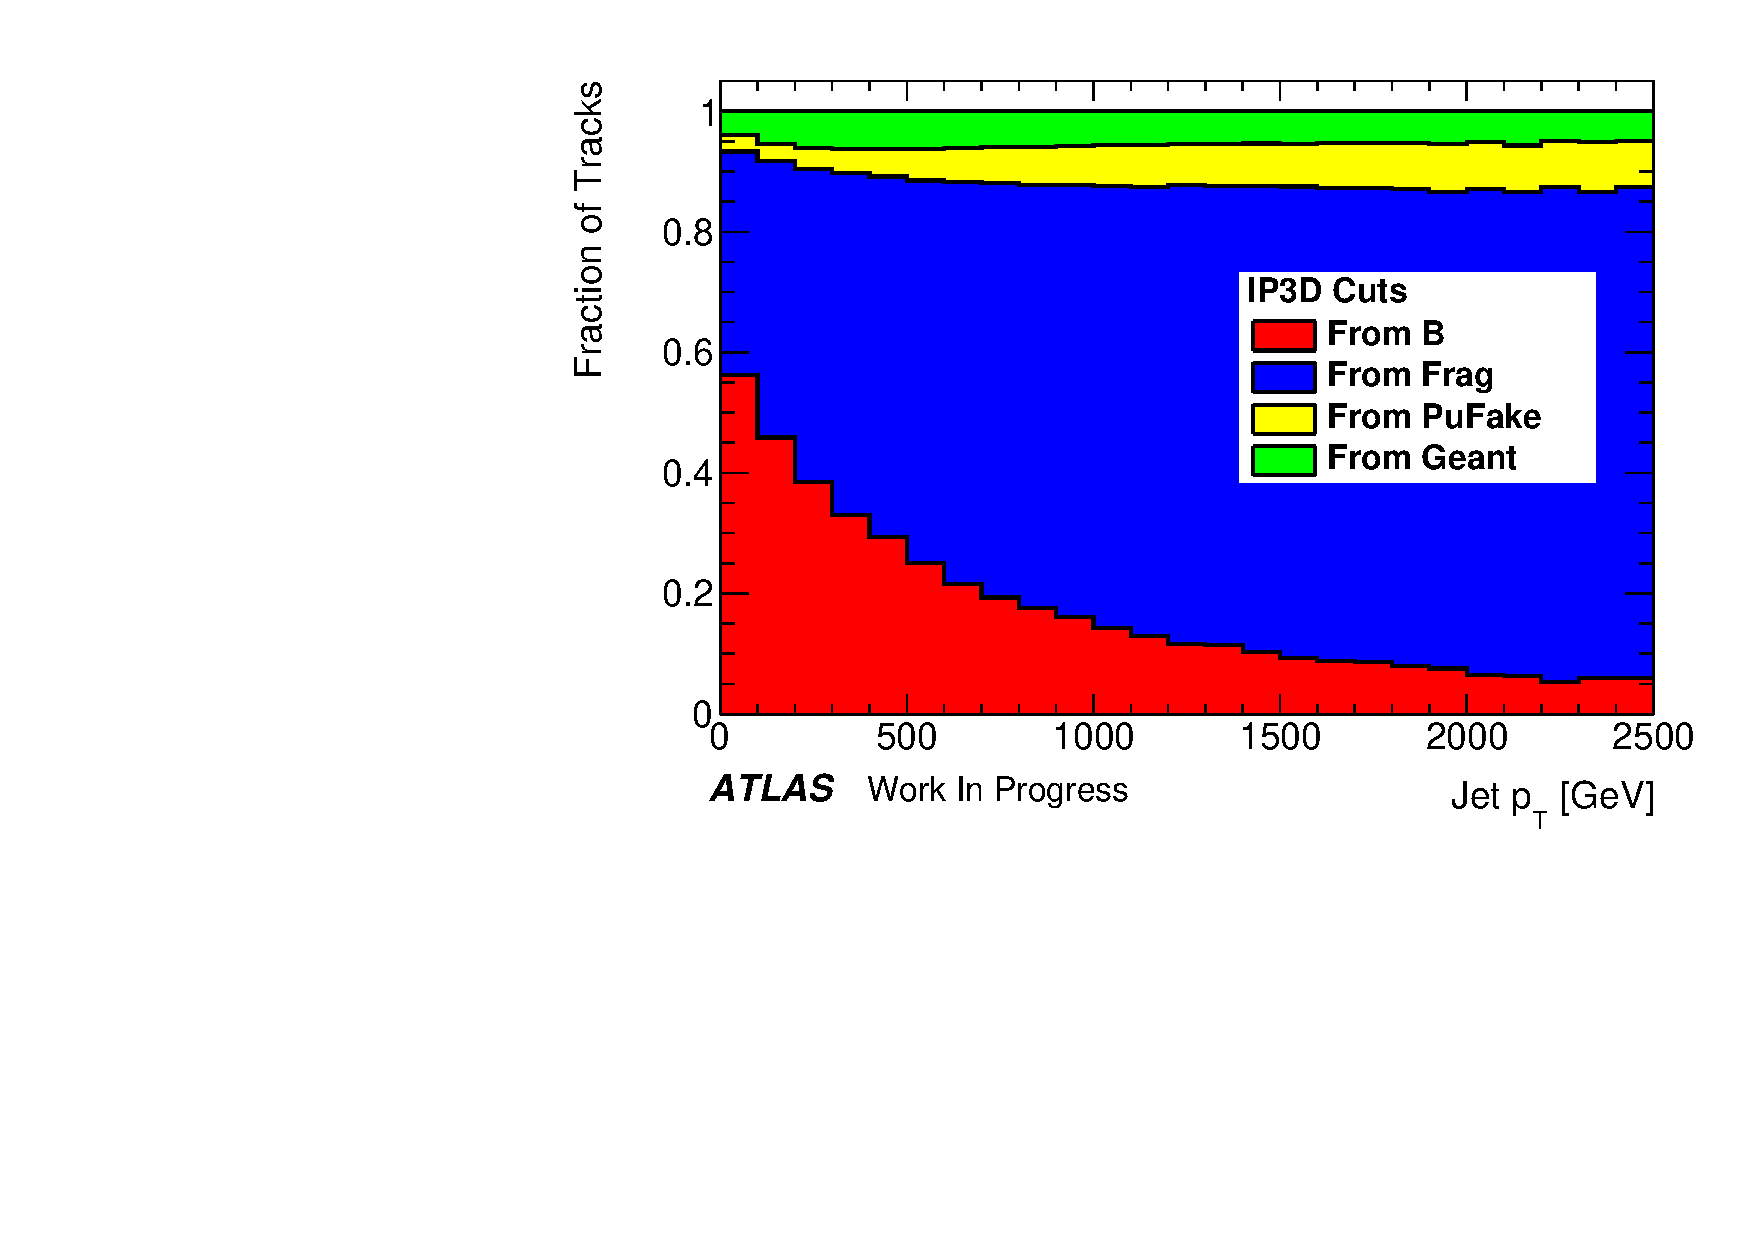
\includegraphics[width=0.45\textwidth]{plots/vpc/frac_IP3D.pdf}
	 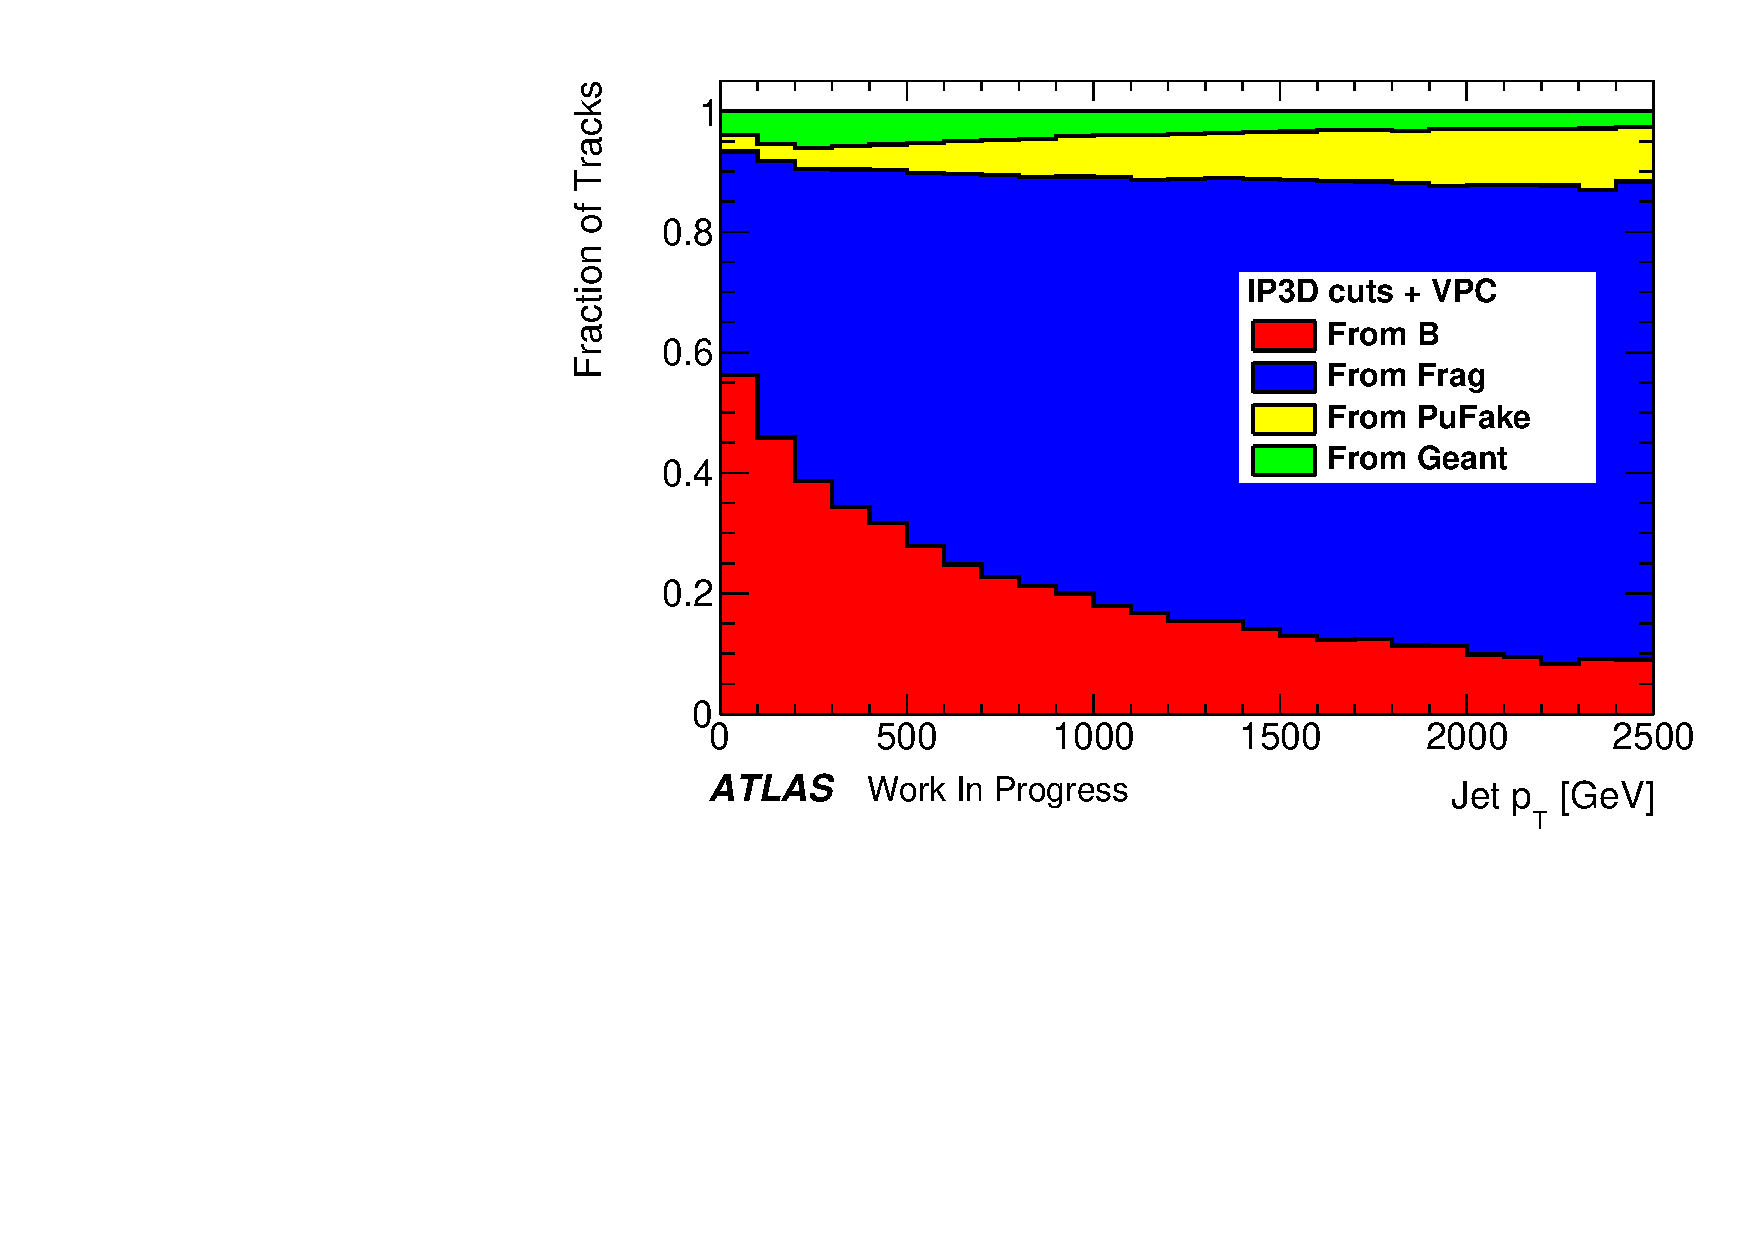
\includegraphics[width=0.45\textwidth]{plots/vpc/frac_vpc.pdf}
	 \caption{The fraction of tracks in a \textit{b}-jet that come from the different track origins when only the IP3D track cuts are applied (left)
           and when the VPC is applied in addition to the IP3D track cuts (right).}
         \label{jet_flav_frac}
\end{figure}


Figure \ref{2D} shows a 2D distribution of track-$p_T$ and jet-$p_T$ for tracks from B (left) and tracks from Fragmentation (right).
The plot has been normalised such that for a given jet-$p_T$ bin, the integral including overfill bins is 1.
The left plot of the figure shows that the $p_T$ of tracks from B increases as jet-$p_T$ increases,
which is due to the strong correlation between jet-$p_T$ and \textit{b}-hadron $p_T$.
In contrast the right plot of the figure shows that many tracks from Fragmentation remain at low track-$p_T$ even at high jet-$p_T$.
Therefore at high jet-$p_T$, there is an opportunity to discriminate between tracks from B and tracks from Fragmentation by considering their track-$p_T$.
In Figure \ref{2D}, the black dotted lines represent the existing track-$p_T >$ 1 GeV cut from the IP3D track cuts,
whilst the magenta line represents a new test track cut, track-$p_T > $
 0.4\% jet-$p_T$, which is referred to as the VPC (variable $p_T$ cut) in this report.   
The VPC is chosen such that it removes the minimal amount of tracks from B, 
whilst also removing the maximum number of tracks from Fragmentation. \\

\begin{figure}[!tb]
	 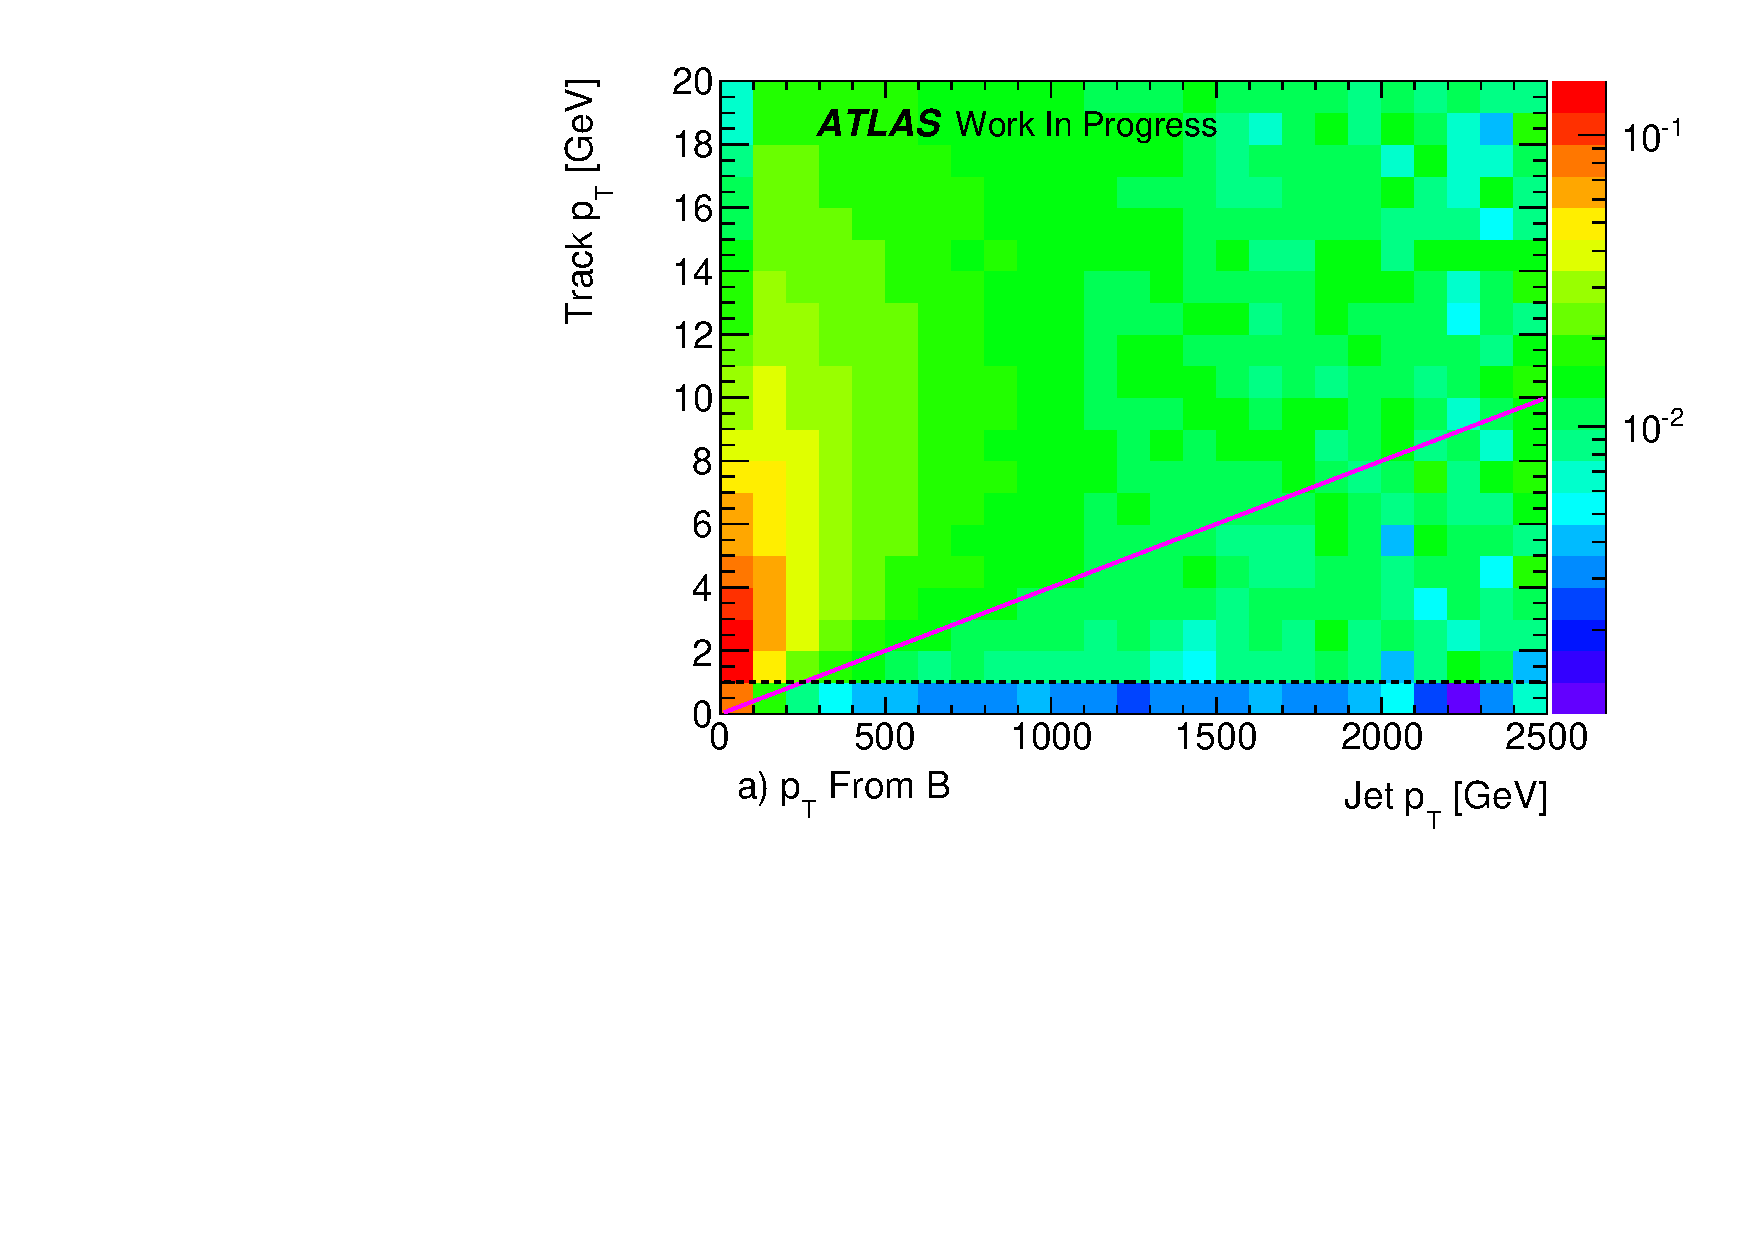
\includegraphics[width=0.45\textwidth]{plots/vpc/2D_B.pdf}
	 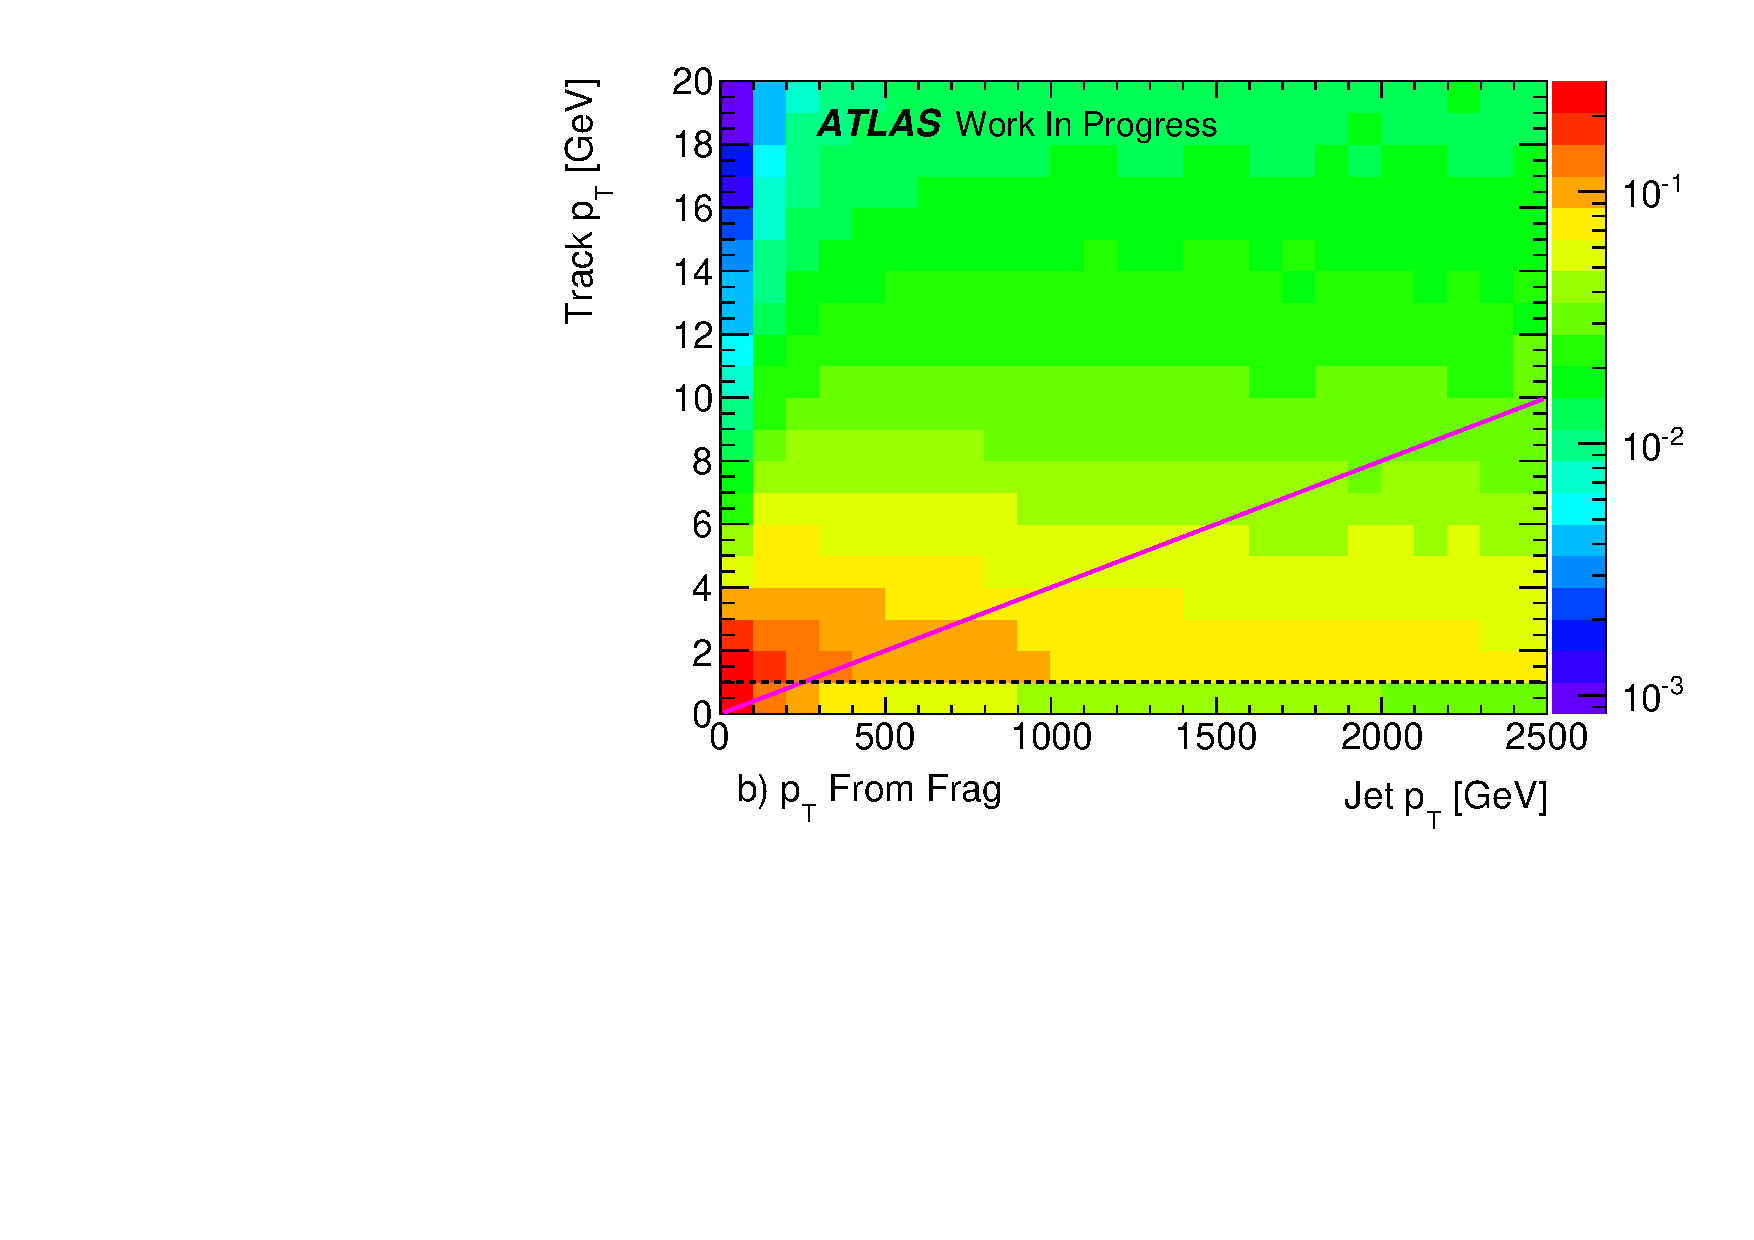
\includegraphics[width=0.45\textwidth]{plots/vpc/2D_Frag.pdf}
	 \caption{A 2D plot to show the distribution of track-$p_T$ against jet-$p_T$ in a \textit{b}-jet for tracks from B (left) and for tracks from Fragmentation (right).
         Each plot such that the slices in jet-$p_T$ integrate to 1.
         The black dotted line represents the track-$p_{T}$ cut in the IP3D track cuts and the magenta line represents the VPC.}
         \label{2D}
\end{figure}


The effect of the VPC can be seen in Figure \ref{eff}, which shows the selection efficiencies of tracks from B and from Fragmentation as a function of jet-$p_T$,
where selection efficiency is defined as 
\begin{equation}
\epsilon_{selection} = \frac{\text{Number of tracks from X selected by set of cuts}}{\text{Truth number of tracks from X}}
\end{equation} 
where X represents one of the track origin categories. 
The red line shows the selection efficiency for the IP3D track cuts, 
whilst the magenta line shows the selection efficiency for the VPC in addition to the IP3D track cuts.
Figure \ref{eff} shows that the addition of the VPC gives a significantly lower selection efficiency of tracks 
from Fragmentation at high jet-$p_T$, whilst the selection efficiency of tracks from B is not strongly affected.
The right plot from Figure \ref{jet_flav_frac} shows the fraction of tracks from each of the track origins when the 
VPC is applied in addition to the IP3D track cuts.
When compared to the left plot of the figure, which shows the same plot when only the IP3D track cuts are applied,
it is shown that the VPC increases the fraction of tracks from B at high jet-$p_T$. 
This shows that the addition of the VPC demonstrates the possibility of improving \textit{b}-tagging at high-$p_T$. \\

\begin{figure}[!bht]
	 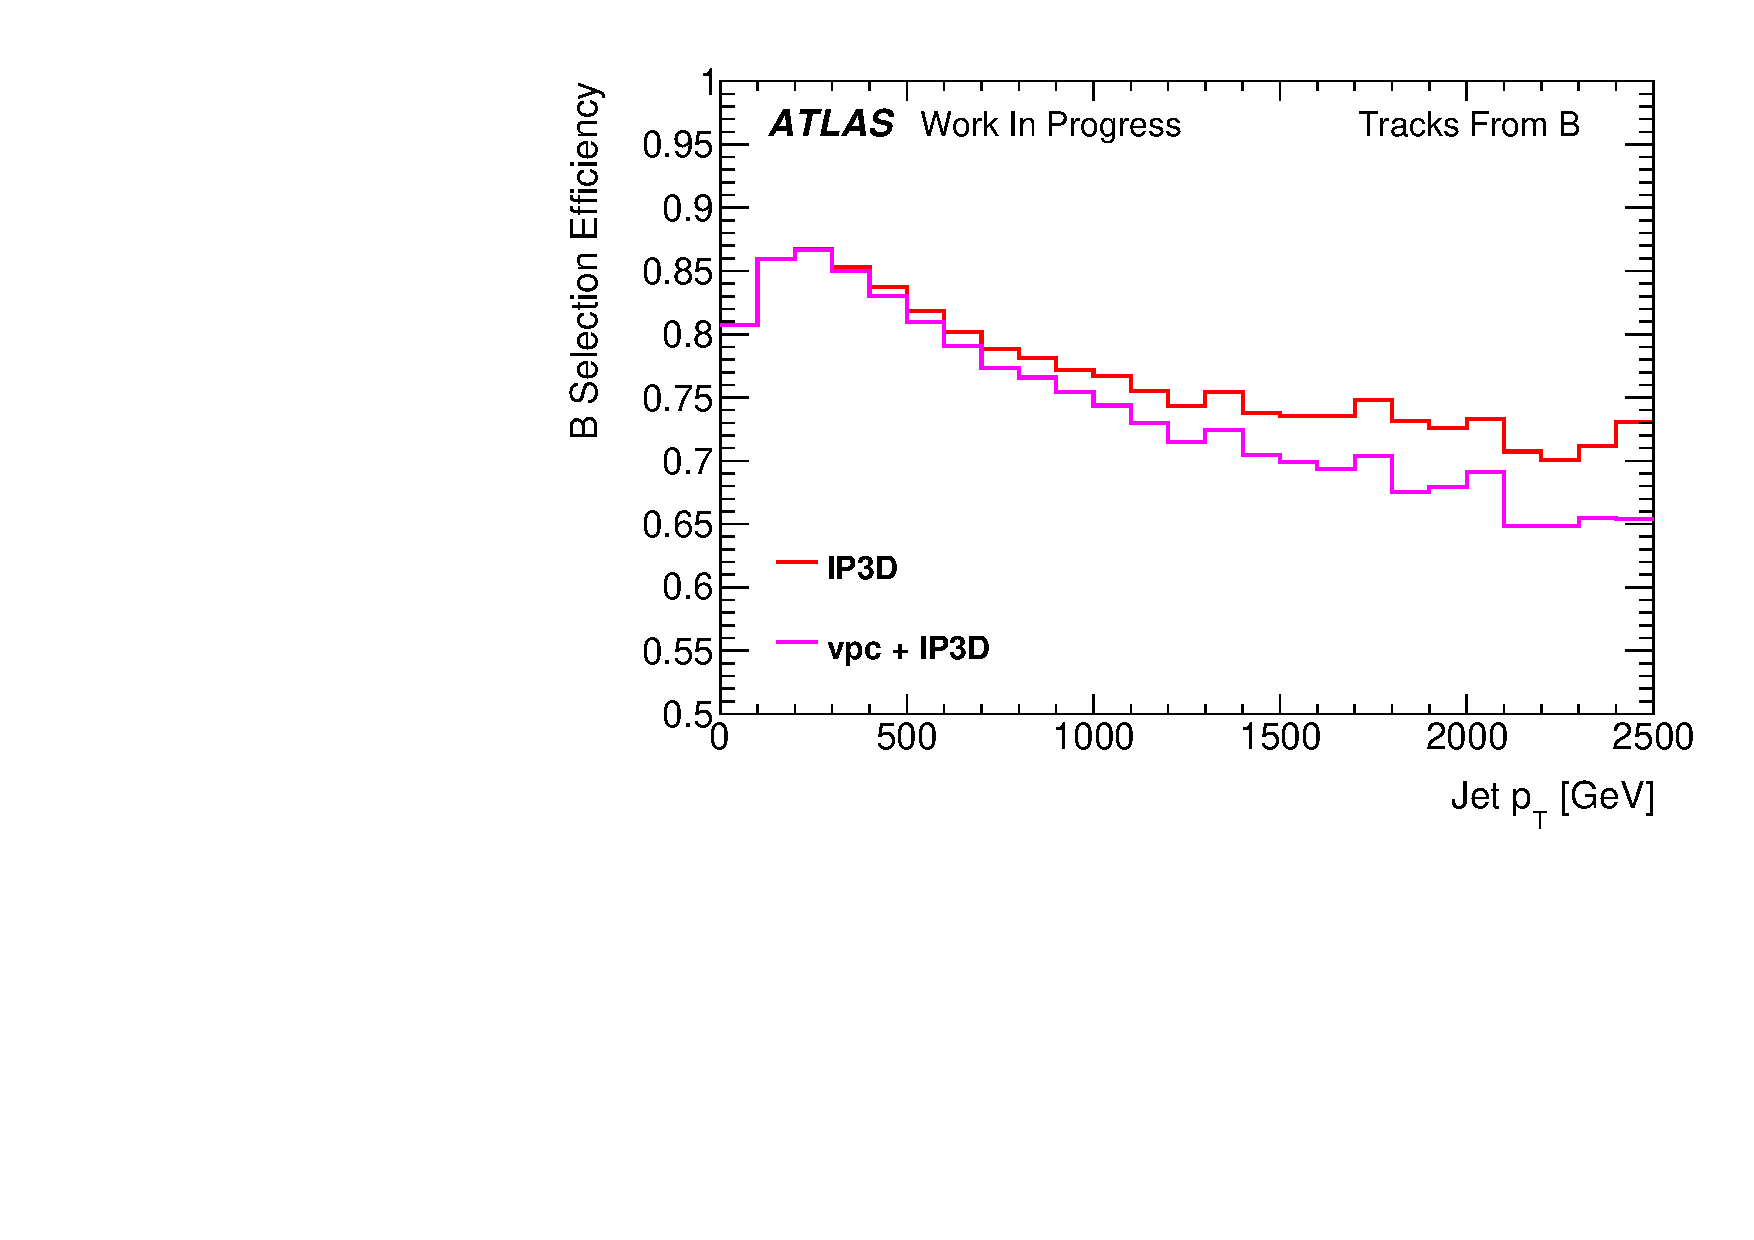
\includegraphics[width=0.45\textwidth]{plots/vpc/effFromB.pdf}
	 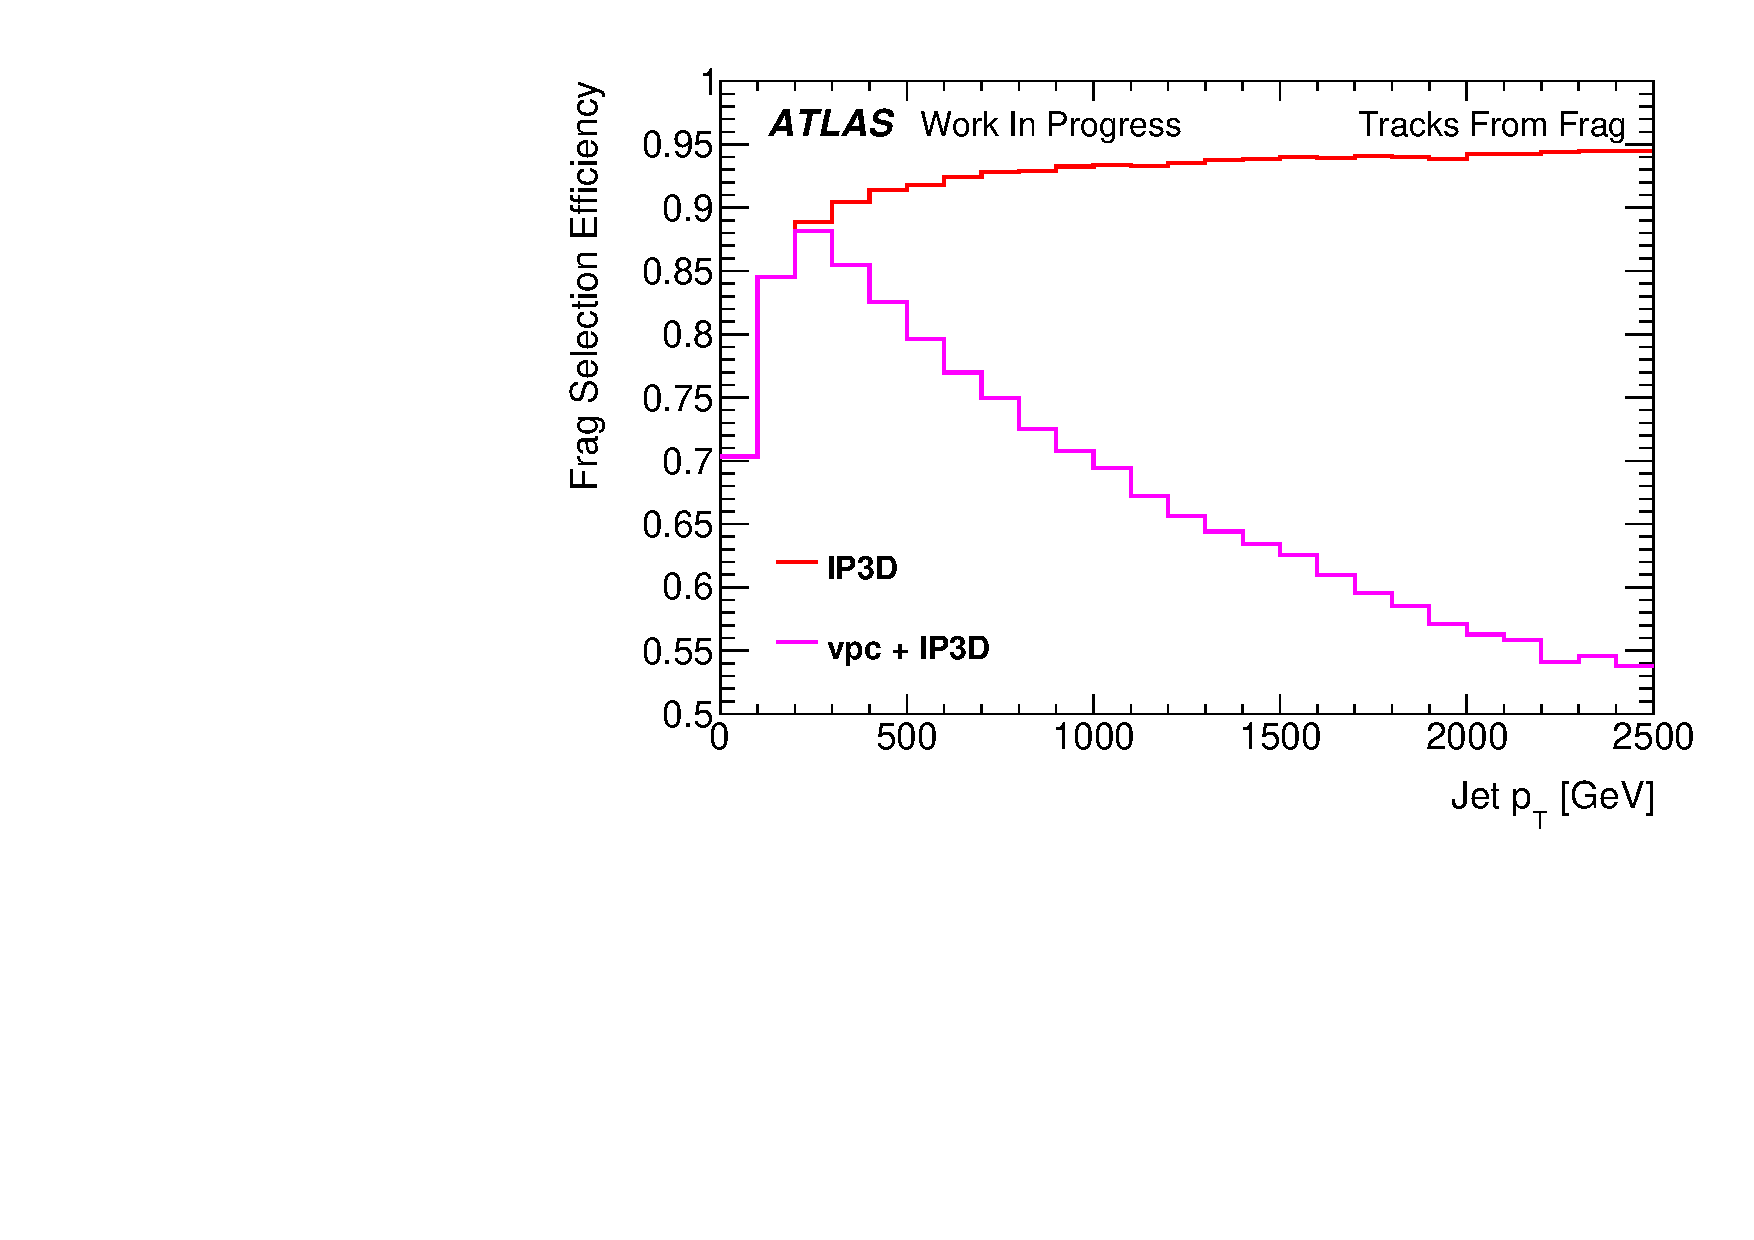
\includegraphics[width=0.45\textwidth]{plots/vpc/effFromFrag.pdf}
	 \caption{The selection efficiency of tracks from B (left) and Fragmentation (right) for IP3D track cuts and VPC in addition to the IP3D track cuts.}
         \label{eff}
\end{figure}


The above discussion is part of an ongoing study to improve high-$p_T$ \textit{b}-tagging performance. 
The next steps of these studies is to implement this study with the full IP3D algorithm to demonstrate that 
the addition of the VPC would improve \textit{b}-tagging performance by producing many ROC curves, 
which would show light-rejection rate against \textit{b}-efficiency, for many different jet-$p_T$ ranges.
It is also necessary to optimise the VPC, by finding the optimal track-$p_T$ cut function to improve light-rejection 
rate for a given \textit{b}-jet efficiency.

\section{Search for Resonances in Di-b-jet Mass Spectrum} \label{s_dibjet}

As discussed in Section \ref{s_ATLAS}, the standard model has a number of inconsistencies with real world observations,
hence there is a requirement for beyond standard model physics.
Run-2 at ATLAS will use pp collisions at the highest centre-of-mass energy ever achieved, 
and hence provides a promising opportunity to search for beyond standard model physics in unexplored
regions of phase space. \\

There are many beyond standard model physics models that predict the existence of massive particles
that decay into pairs of quarks and gluons \cite{bib_qstar, bib_W', bib_W*, bib_color_octet}.
Previously, searches have been performed for these massive particles at ATLAS and other experiments by looking for resonances in the
distribution of the invariant mass of the leading and subleading jets, known as the dijet mass spectrum or $m_{jj}$ \cite{bib_ATLAS_dijet, bib_dijet}.
The smoothly falling function given below, has been shown in the previous studies to fit the QCD dijet background:
\begin{equation}
  f(x) = p_1(1-x)^{p_2}x^{p_3+p_4\text{ln}(x)}
  \label{dijet_fit}
\end{equation}
where $p_i$ are fit parameters and $x \equiv m_{jj}/\sqrt{s}$. 
Hence this function is used to fit the QCD dijet background,
 then any significant excesses above this background, 
which could be representative of a resonance, are then identified.
 
\begin{figure}[!bht]
  \begin{center}
	 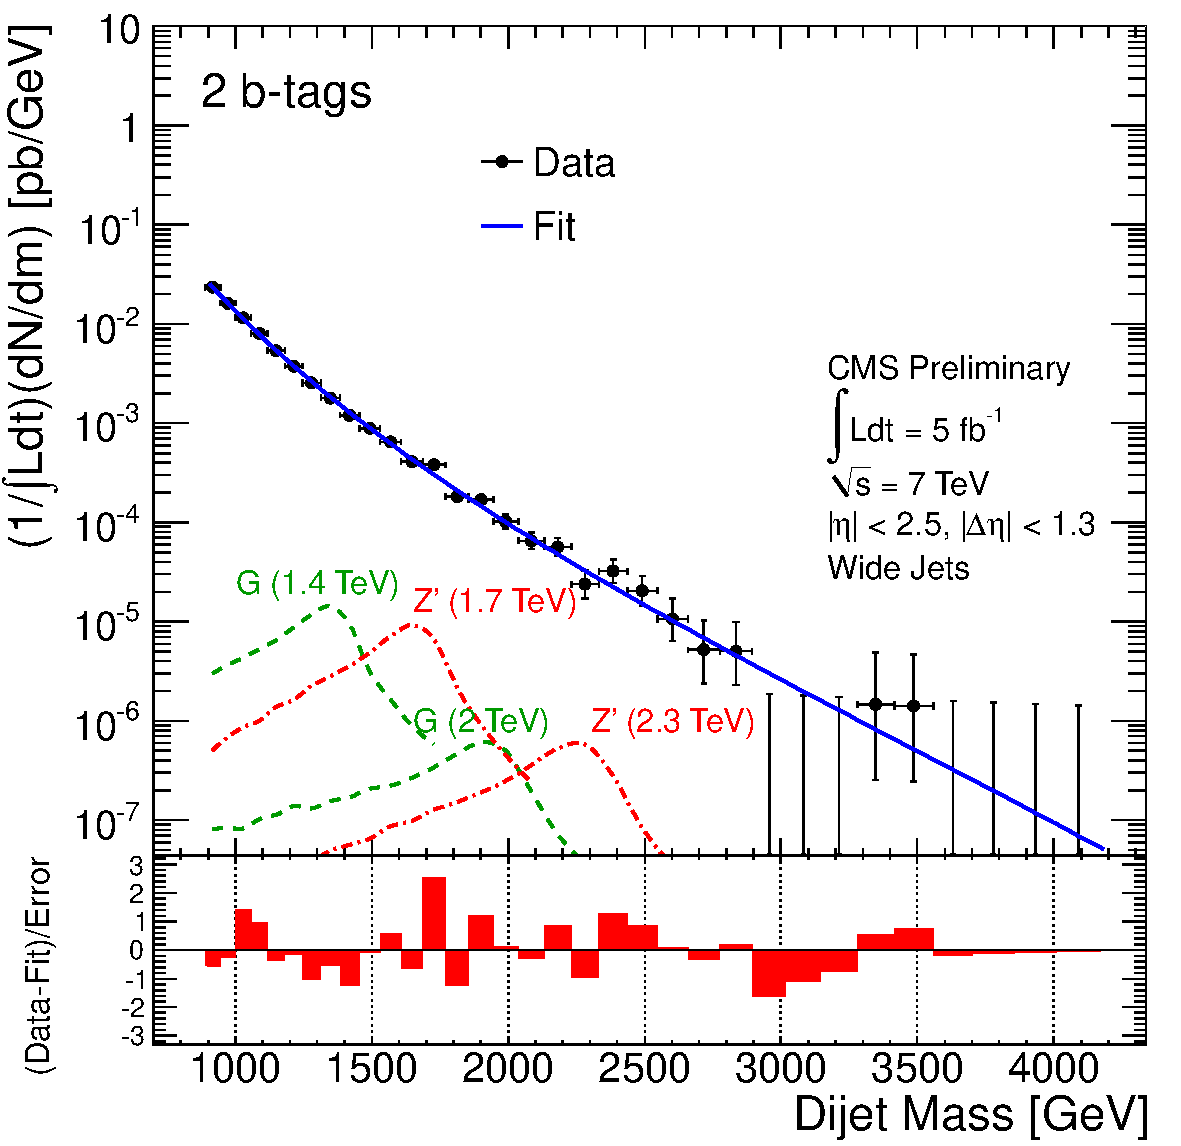
\includegraphics[width=0.4\textwidth]{figures/CMS_dibjet.pdf}
	 \caption{The dijet mass spectrum of two \textit{b}-tagged jets (points) compared to a smooth fitting function (solid line)
           Predictions for the Z'-boson (dot-dashed) and a RS graviton (dashed) are shown.}
         \label{CMS_dibjet}
         \vspace{-0.2cm}
  \end{center}
\end{figure}


In addition, there are many similar models that predict a decay into two \textit{b}-quarks,
an example is the sequential standard model Z'-boson, which is predicted by many models with new gauge symmetries \cite{bib_Z'}.
Assuming that the Z'-boson has the same couplings to SM particles as the Z-boson, the ratio of the branching fraction
of Z'-boson decaying to $b\bar{b}$ to the branching fraction of the Z'-boson decaying to $q\bar{q}$ of any flavour is approximately 0.22,
Hence, given that the QCD dijet background is dominated by light jets, 
by considering the dijet spectrum of two \textit{b}-tagged jets one can improve the sensitivity to the models 
with that decay into two \textit{b}-quarks.
Searches for resonances in the dijet spectrum of \textit{b}-tagged jets has occurred at CMS in $\sqrt{s}$ = 7 TeV collisions,
the dijet spectrum is shown in Figure \ref{CMS_dibjet} \cite{bib_CMS_dibjet}.
No significant excesses from background were found and a limit on Acceptance x Cross-section 
of an object decaying into $b\bar{b}$ is placed. \\

A similar analysis is planned in Run-2 data from ATLAS, which, due to the higher centre-of-mass energy ($\sqrt{s} =$ 13 TeV), 
will be able to search for resonances in new regions of phase space.
An important feature of this analysis will understanding and improving \textit{b}-tagging at high jet-$p_T$. 
It is important that any sculpting of the dijet mass spectrum caused by a non-smooth efficiency profile of 
high-$p_T$ \textit{b}-tagging is well understood.
A further discussion of high-$p_T$ \textit{b}-tagging is found in Section \ref{s_high_pt_btag}.

\section*{Summary and Future Outlook}

There have been many changes between Run-1 and Run-2 that have an effect on flavour tagging performance.
The understanding of these changes to flavour tagging performance gained in simulation has been validated in early
Run-2 data by comparing the key variables relevant to \textit{b}-tagging in data and simulation in an inclusive dijet sample.
There are variables that show reasonable agreement; the jet-kinematics, the variables from SV and JF,
and MV2c20 for a sample that is enhanced in \textit{b}-jets.
There are also some variables where there is disagreement; the impact parameter distributions and the MV2c20 distribution for the full sample.
Further investigations are required to understand the differences between data and simulation. \\

In addition an ongoing-study of track selection of the IP3D algorithm at high jet $p_T$ has been presented.
It has been shown that introducing a track-$p_T$ cut that depends on jet-$p_T$, 
in addition to the track cuts that are already applied by the IP3D algorithm,
increases the fraction of tracks that originate from the decay of a \textit{b}-hadron used by the IP3D algorithm,
which may in turn increase the \textit{b}-tagging performance.
The next steps for this study are to demonstrate that the addition of the jet-$p_T$ dependant cut improves \textit{b}-tagging performance by 
producing ROC curves, that show \textit{b}-jet efficiency against light-rejection rates, for different jet-$p_T$ bins.
ROC curves can also be used to optimise this cut, by trialling several different cut functions, and finding the cut function that optimises flavour tagging performance. \\

Finally, a proposed analysis searching for particles that decay into $b\bar{b}$ using
the dijet mass spectrum of two \textit{b}-tagged jets in Run-2 data at ATLAS has been discussed in this report.
By searching for significant discrepancies above the QCD background in the dijet spectrum, one is sensitive to beyond standard model physics,
such as a Z'-boson.
Improvements in high jet-$p_T$ \textit{b}-tagging will significantly increase the sensitivity of this analysis. 

\newpage
\bibliography{UCL_FirstYearReport}
\bibliographystyle{unsrt}
\end{document}
